\section{Performance Evaluation}
\label{sec:results}

This section describes the experimental evaluation of the strategy proposed to redirect the users, including the scenarios, metrics, methodology, and outcomes.
 
%\subsection{Methodology}
%
%We present three approaches to address the methodological problems identified in a edge/cloud multi-tier network for watching a video streaming: cloud-only 

\subsection{Experimental Setup}

%[29] Christian Kreuzberger, Daniel Posch, and Hermann Hellwagner. Amust framework - adaptive multimedia streaming simulation framework for ns-3 and ndnsim, 2016.
%[30] C. Mueller, S. Lederer, J. Poecher, and C. Timmerer. Demo paper: Libdash - an open source software library for the mpeg-dash standard. In 2013 IEEE International Conference on Multimedia and Expo Workshops (ICMEW), pages 1–2, July 2013.
% Per-title encode optimization, 2015. ; accessed 20-novembro-2019.

We use Adaptive Multimedia Streaming~(AMuSt)~\cite{kreuzberger2016amust} to implement a video streaming server, and the server is implemented through Dynamic Adaptive Streaming over HTTP~(DASH) and users that allow adaptive video streaming. The AMuSt framework provides a set of applications for producing and consuming adaptable videos based on the DASH standard. DASH functionality is provided by the libdash library~\cite{mueller2013ICMEW}, an open source library that provides an interface to the DASH standard. Currently, libdash is the official reference software for the DASH standard. We consider that users are interested in an available video with ten different bit rate representations \{235kbps, 375kbps, 560kbps, 560kbps, 750kbps, 1050kbps, 1750kbps, 2350kbps, 3000kbps, 4300kbps, 5800kbps\}, which are used by Netflix subsets~\cite{netflix:representation}, which Netflix uses. [31]. Each representation is divided into 2-second segments. Each experiment is executed once with a video of 1600 seconds~(800 segments). 
For the sake of simplicity, the multimedia content used in the simulation is already deployed in the edge peering nodes. 

%Figure 3 shows the topology with three levels used in the experiments, each level \{1, 2 and 3\} is represented as a scenario.

%Dash server and the clients allowed to request a multimedia content in DASH format, was used the Adaptive Multimedia Streaming~(AMuSt). The AMust system allow a set o apps to produce and consume the adaptive video, based on Dash pattern. The DASH functionality is provided by the libdash library, an open source library that provides an interface to the DASH standard. Currently, libdash is the reference software official DASH standard.

We simulate the scenario in a binary tree topology with seven nodes and a Cloud Provider connected to the root node of the Binary tree. The last four nodes are Access Points~(AP), and the others are edge peering points. Figure~\ref{fig:exp-setup-scenario} illustrate the binary tree scenario.

The AP nodes are implemented on a wireless device that communicates via IEEE 802.11g in 2.4GHz frequency. The APs are connected to the edge peering points by wire and the end-users via wireless. Each user connected to the AP is located precisely 8 meters away. The Bandwidth available in each link can seem in Fig.~\ref{fig:exp-setup-scenario}.

We present three approaches to address the impacts identified in Section~\ref{sec:system-archi} into the edge/cloud multi-tier network: the \textit{cloud-only}, \textit{1\&2 nodes} and mobile-based scenarios. The cloud-only scenario uses just the Cloud Provider node to deliver the video content. \textit{1\&2 nodes} uses nodes 1 and 2 as auxiliary nodes to deliver the video. The simulation starts with the users requesting the video from the cloud. When some link detects a congested link, the edge cache below the link is turned on. Thereafter, the users receiving the video over the congested link are redirected to the edge node. 

The number of end-user devices communicating through each wireless AP may change over time due to the mobility of the end-user devices. In practice, the number of end-user devices connecting to the wireless AP changes frequently. 
To show the problems that can appear in such scenarios, and a connection change between the APs occurs. We reran the second experiment, maintaining connections between users and edge nodes, but changed the connection between users and APs. Where half the users of each $AP_{i}$ go directly to $AP_{i + 2}$.
%Onde os metade dos usuários de cada $AP_{i}$ vão diretamente para o $AP_{i+2}$.
%Para mostrar os problemas que podem aparecer em tais cenários, e ocorre uma mudança de conexão entre os APs. Nós executamos novamente o segundo experimento mantendo as conexões entre os usuários e edge nodes, mas mudamos a conexão entre os usuários e os APs. 


\begin{figure}
    \centering
    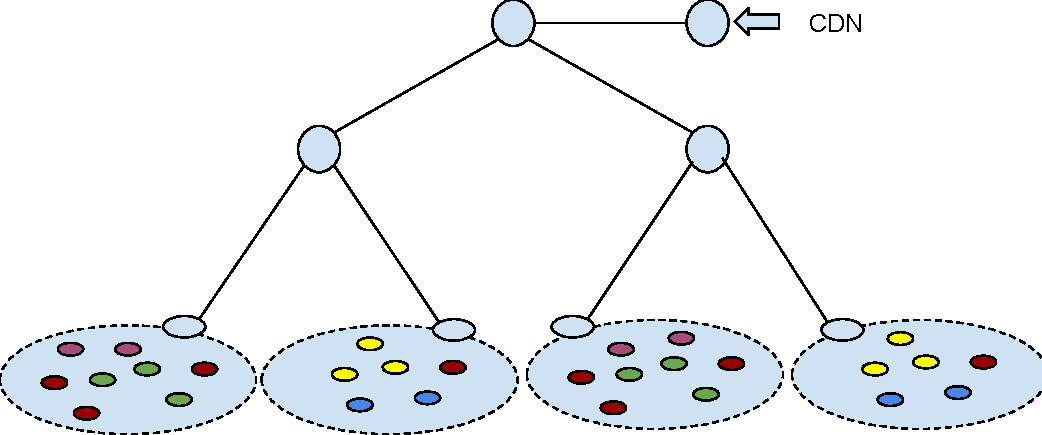
\includegraphics[width=0.9\linewidth]{images/exp-setup-scenario.pdf}
    \caption{A General Overview of the multi-tier network environment.}
    \label{fig:exp-setup-scenario}
\end{figure}

%To illustrate the idea, we assume tree topology. According to the guideline, a mobile backhaul network is modeled as a two-level hierarchical network. Wireless base stations are connected to aggregation nodes, e.g., service/packet data network gateway (S/P-GW) nodes. Furthermore, aggregation nodes are connected to core nodes, e.g., central office nodes. To the best of our knowledge, separation of traffic from one wireless base stations to multiple aggregation nodes, and from one aggregation node to multiple core nodes is not dominant in current mobile backhaul networks. Thus, we assume a tree-topology backhaul network


\subsection{QoE Metric evaluation}

There exist many viewer QoE models in the literature. We will describe the QoE metrics used to score user satisfaction. Firstly, We compute each video quality chunk by a logarithmic law over bitrates~\cite{Reichl:TSys2013}. The study proposes a video quality model for DASH, as shown in Equation (1). Each video has $N$ segments and is encoded with $L$ bitrate levels. $r_i$ represents a specific bitrate level. At each step $i$, the quality of segment $i$, which is encoded at $l_i$ is defined as:

$$
q(r_i) = a_1 * log(a_2 * (r_i/ r_{|L|}))
$$

We require a flexible QoE model that includes the most influential metrics to quantify long-term users' QoE. 
We consider the Eq.~\ref{eq:qoe-equation} which consists of four metrics: (a) the average chunk perceptual quality, (b) the average number of quality oscillations, (c) the average number of stall events and their durations, and (d) the startup delay. $K$ represents the total segments of the video, $S_{i}$ is the stall duration, and $ST_{i}$ is the startup delay of user $i$.

\begin{equation}\label{eq:qoe-equation}
\begin{split}
QoE_i = \frac{1}{K} \sum_{k=1}^{K}q(r_{k}) - \frac{1}{K-1} \sum_{k=1}^{K-1}|q(r_{k+1}) - q(r_{k}))| \\
- \frac{1}{K}\sum_{k=1}^{K} S_{k} - ST_{i}
\end{split}
\end{equation}

The $QoE_{i}$ for each user $i$ has a range of 1 to 5. Where the values 1 = bad, 2 = poor, 3 = fair, 4 = good, and 5 = excellent.


% \begin{figure*}
%     \centering
%     \subfigure[]{
%     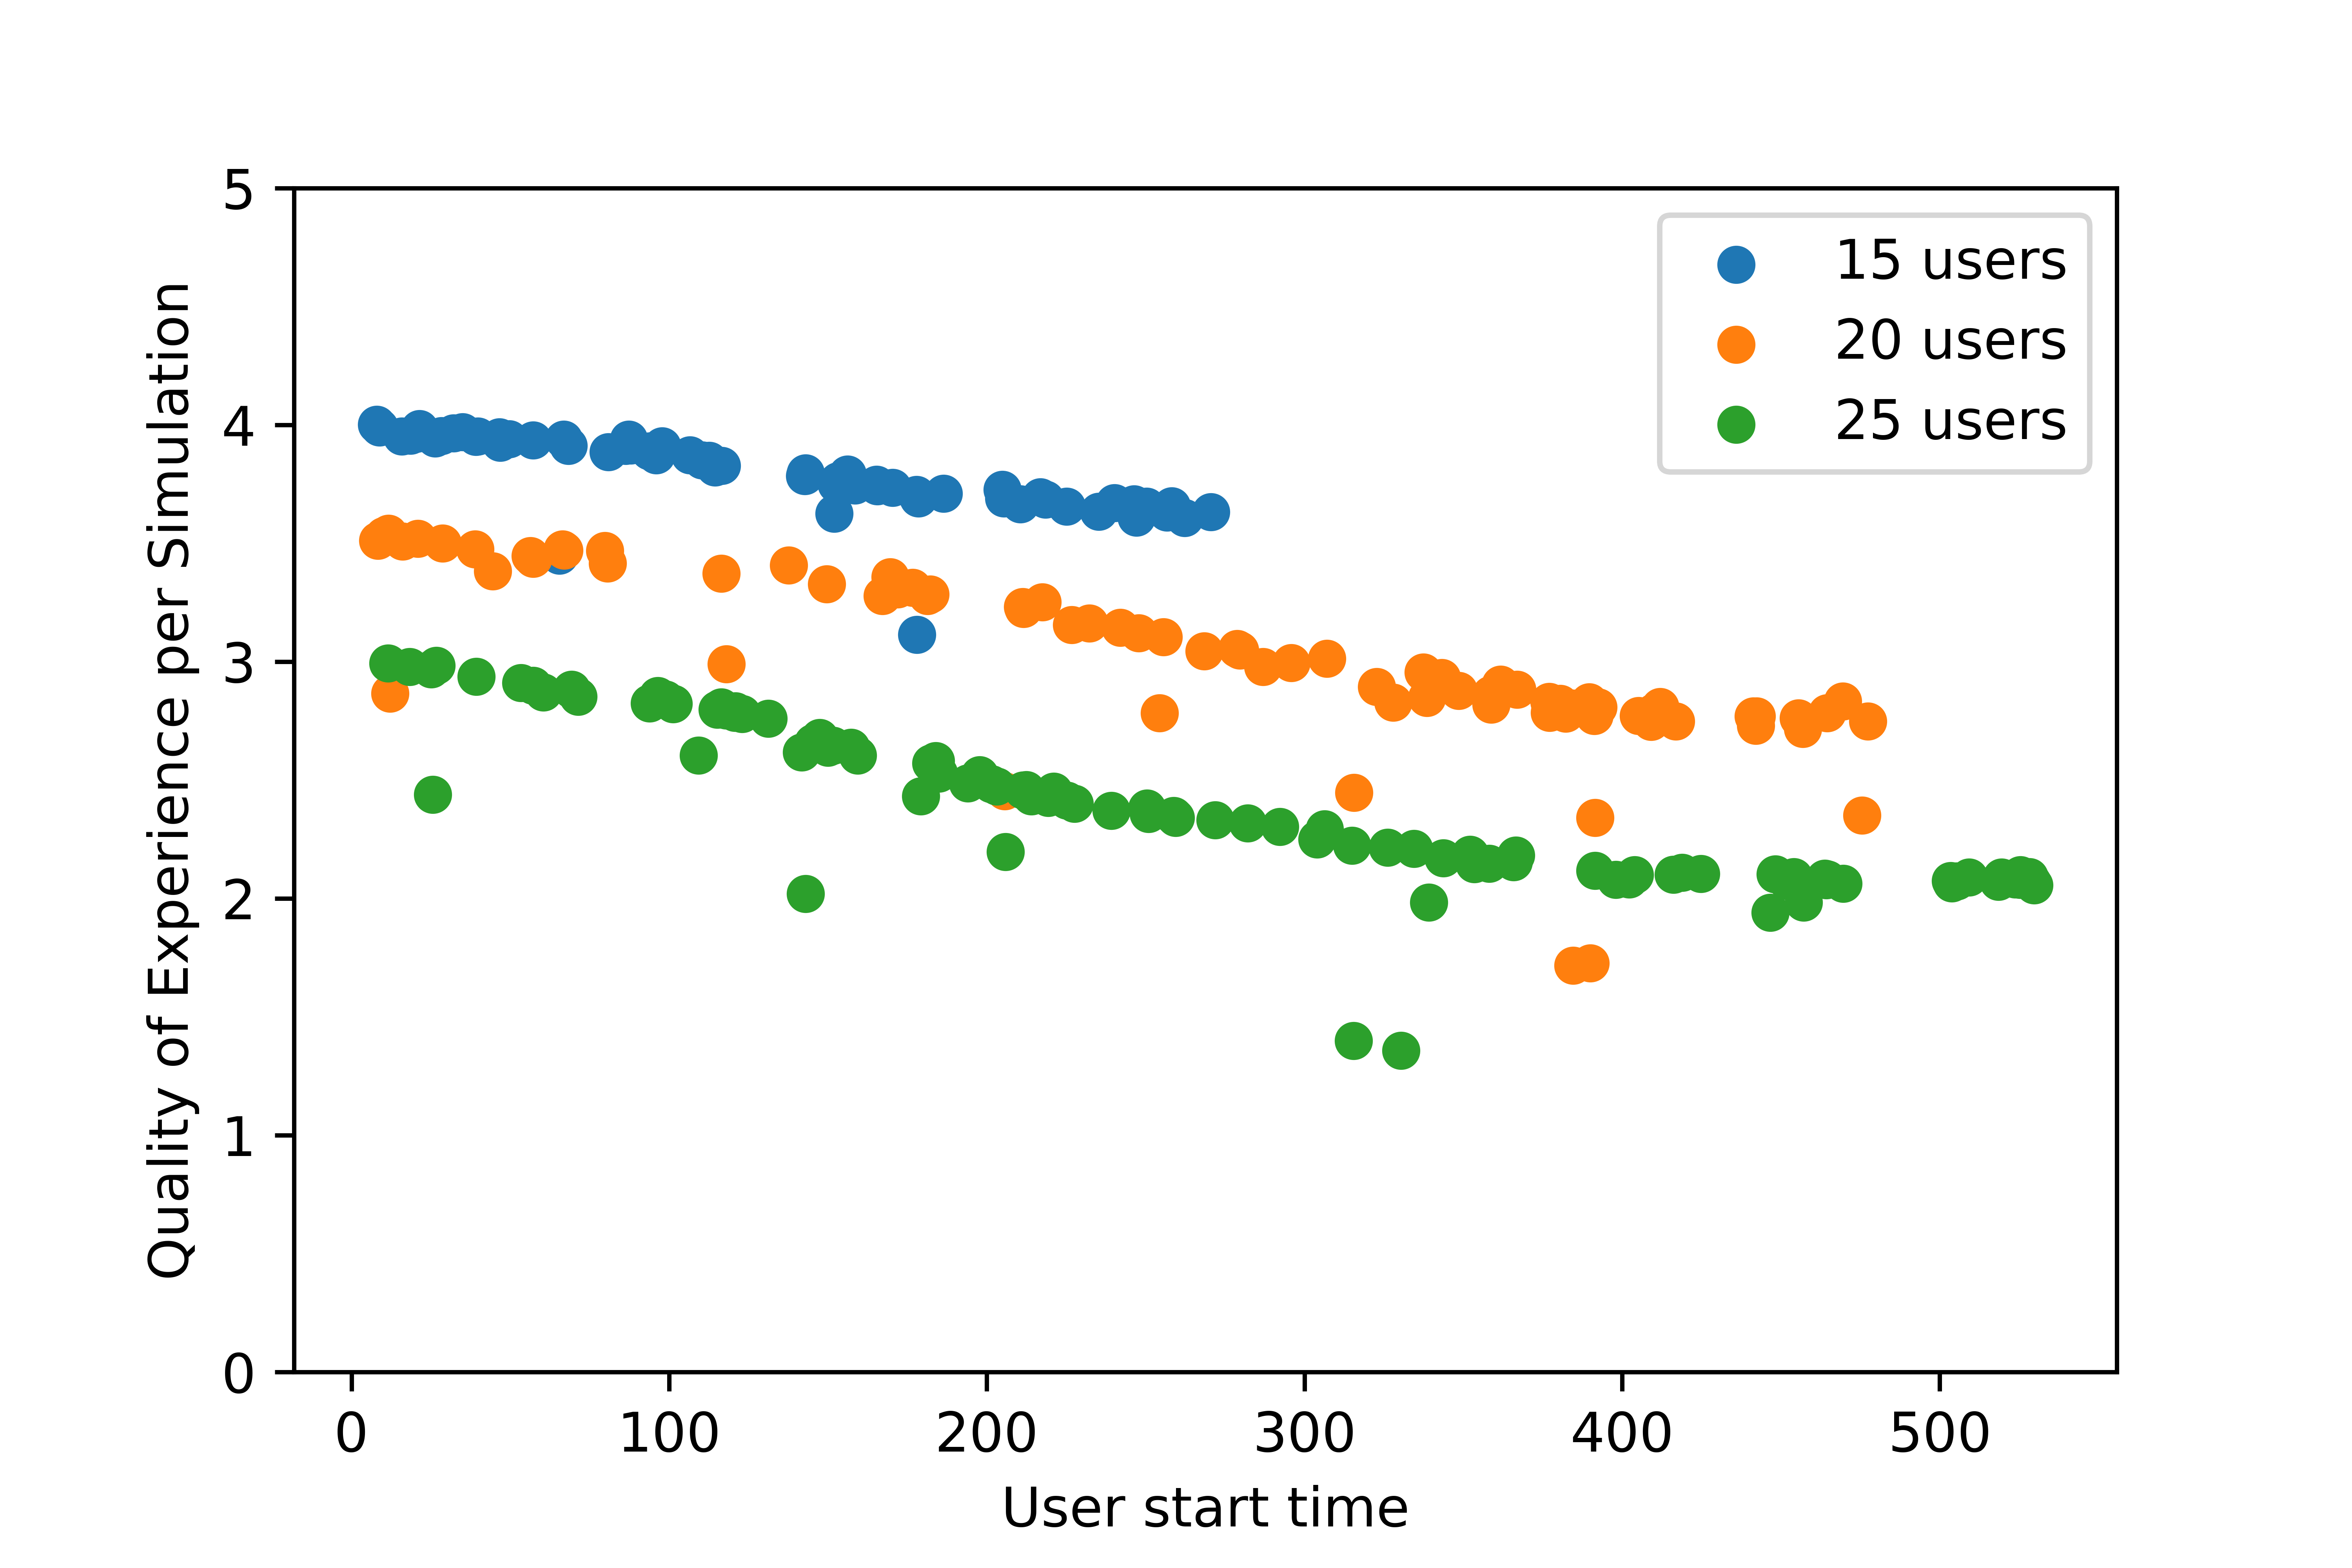
\includegraphics[width=0.45\linewidth]{images/QoECompare.png}
%     \label{fig:red-comparison-plot}
%     }
%     \subfigure[]{
%     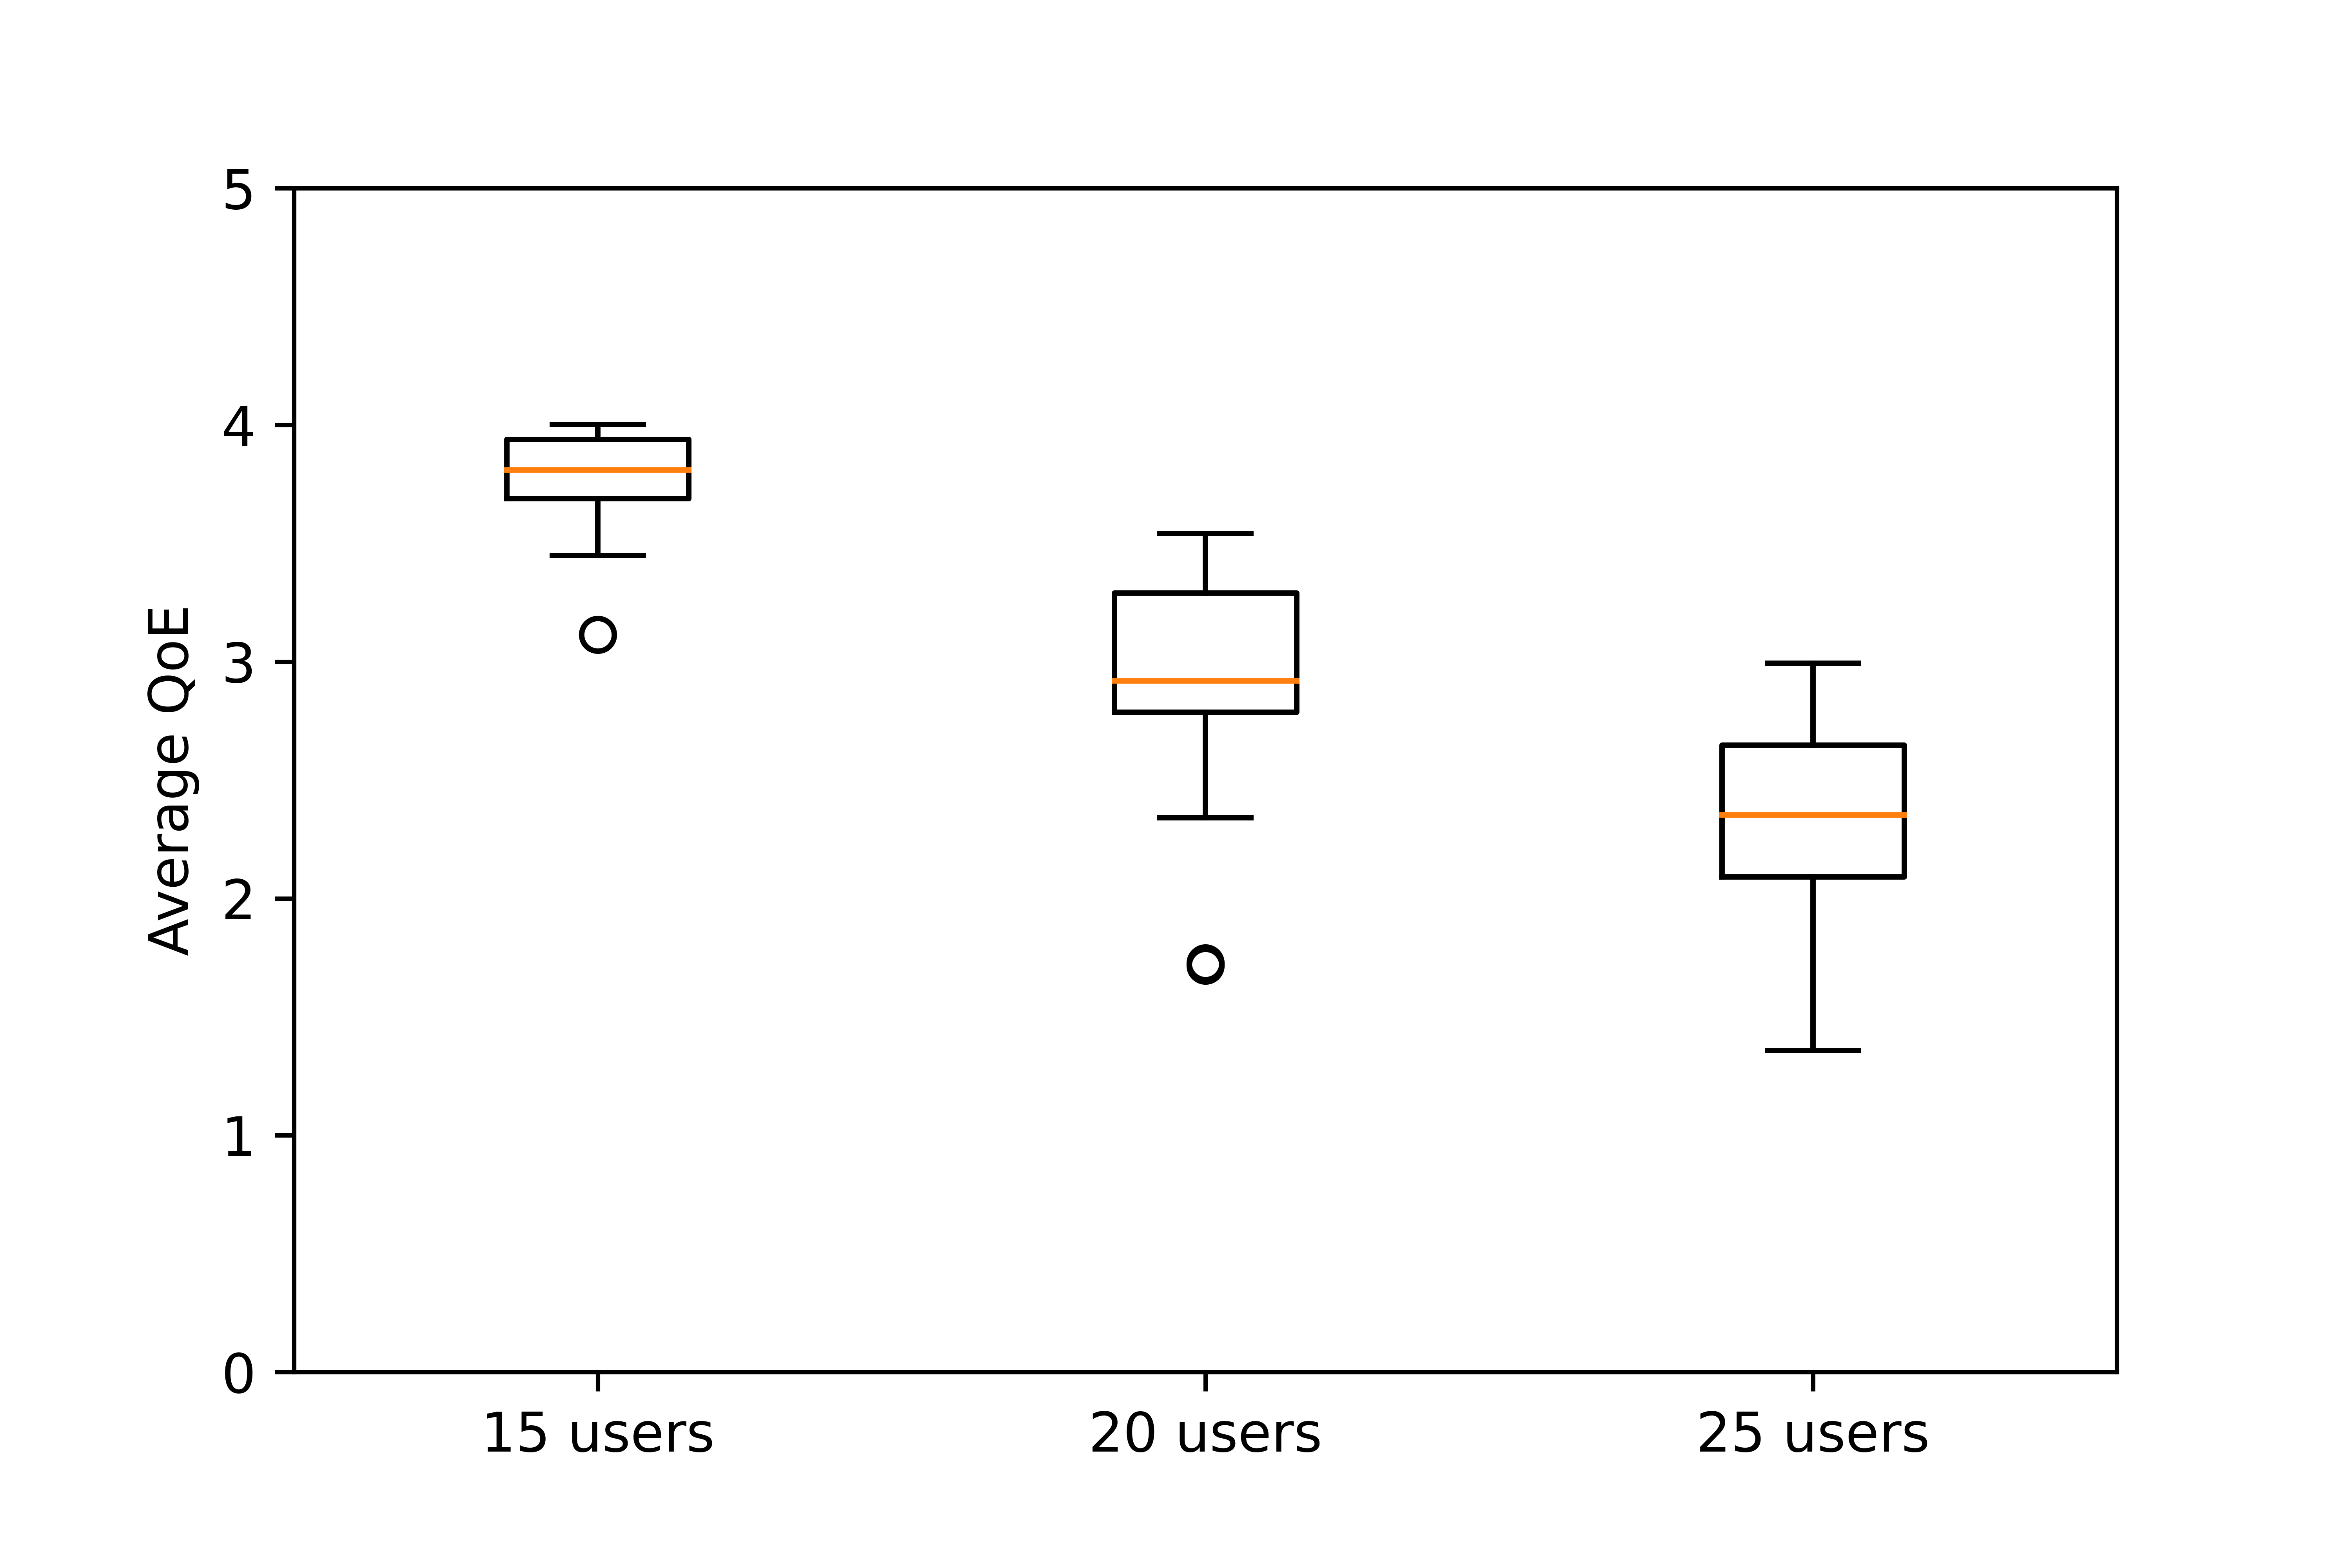
\includegraphics[width=0.45\linewidth]{images/QoEBoxplot.png}
%     \label{fig:co-comparison-boxplot}
%     }

%     \subfigure[]{
%     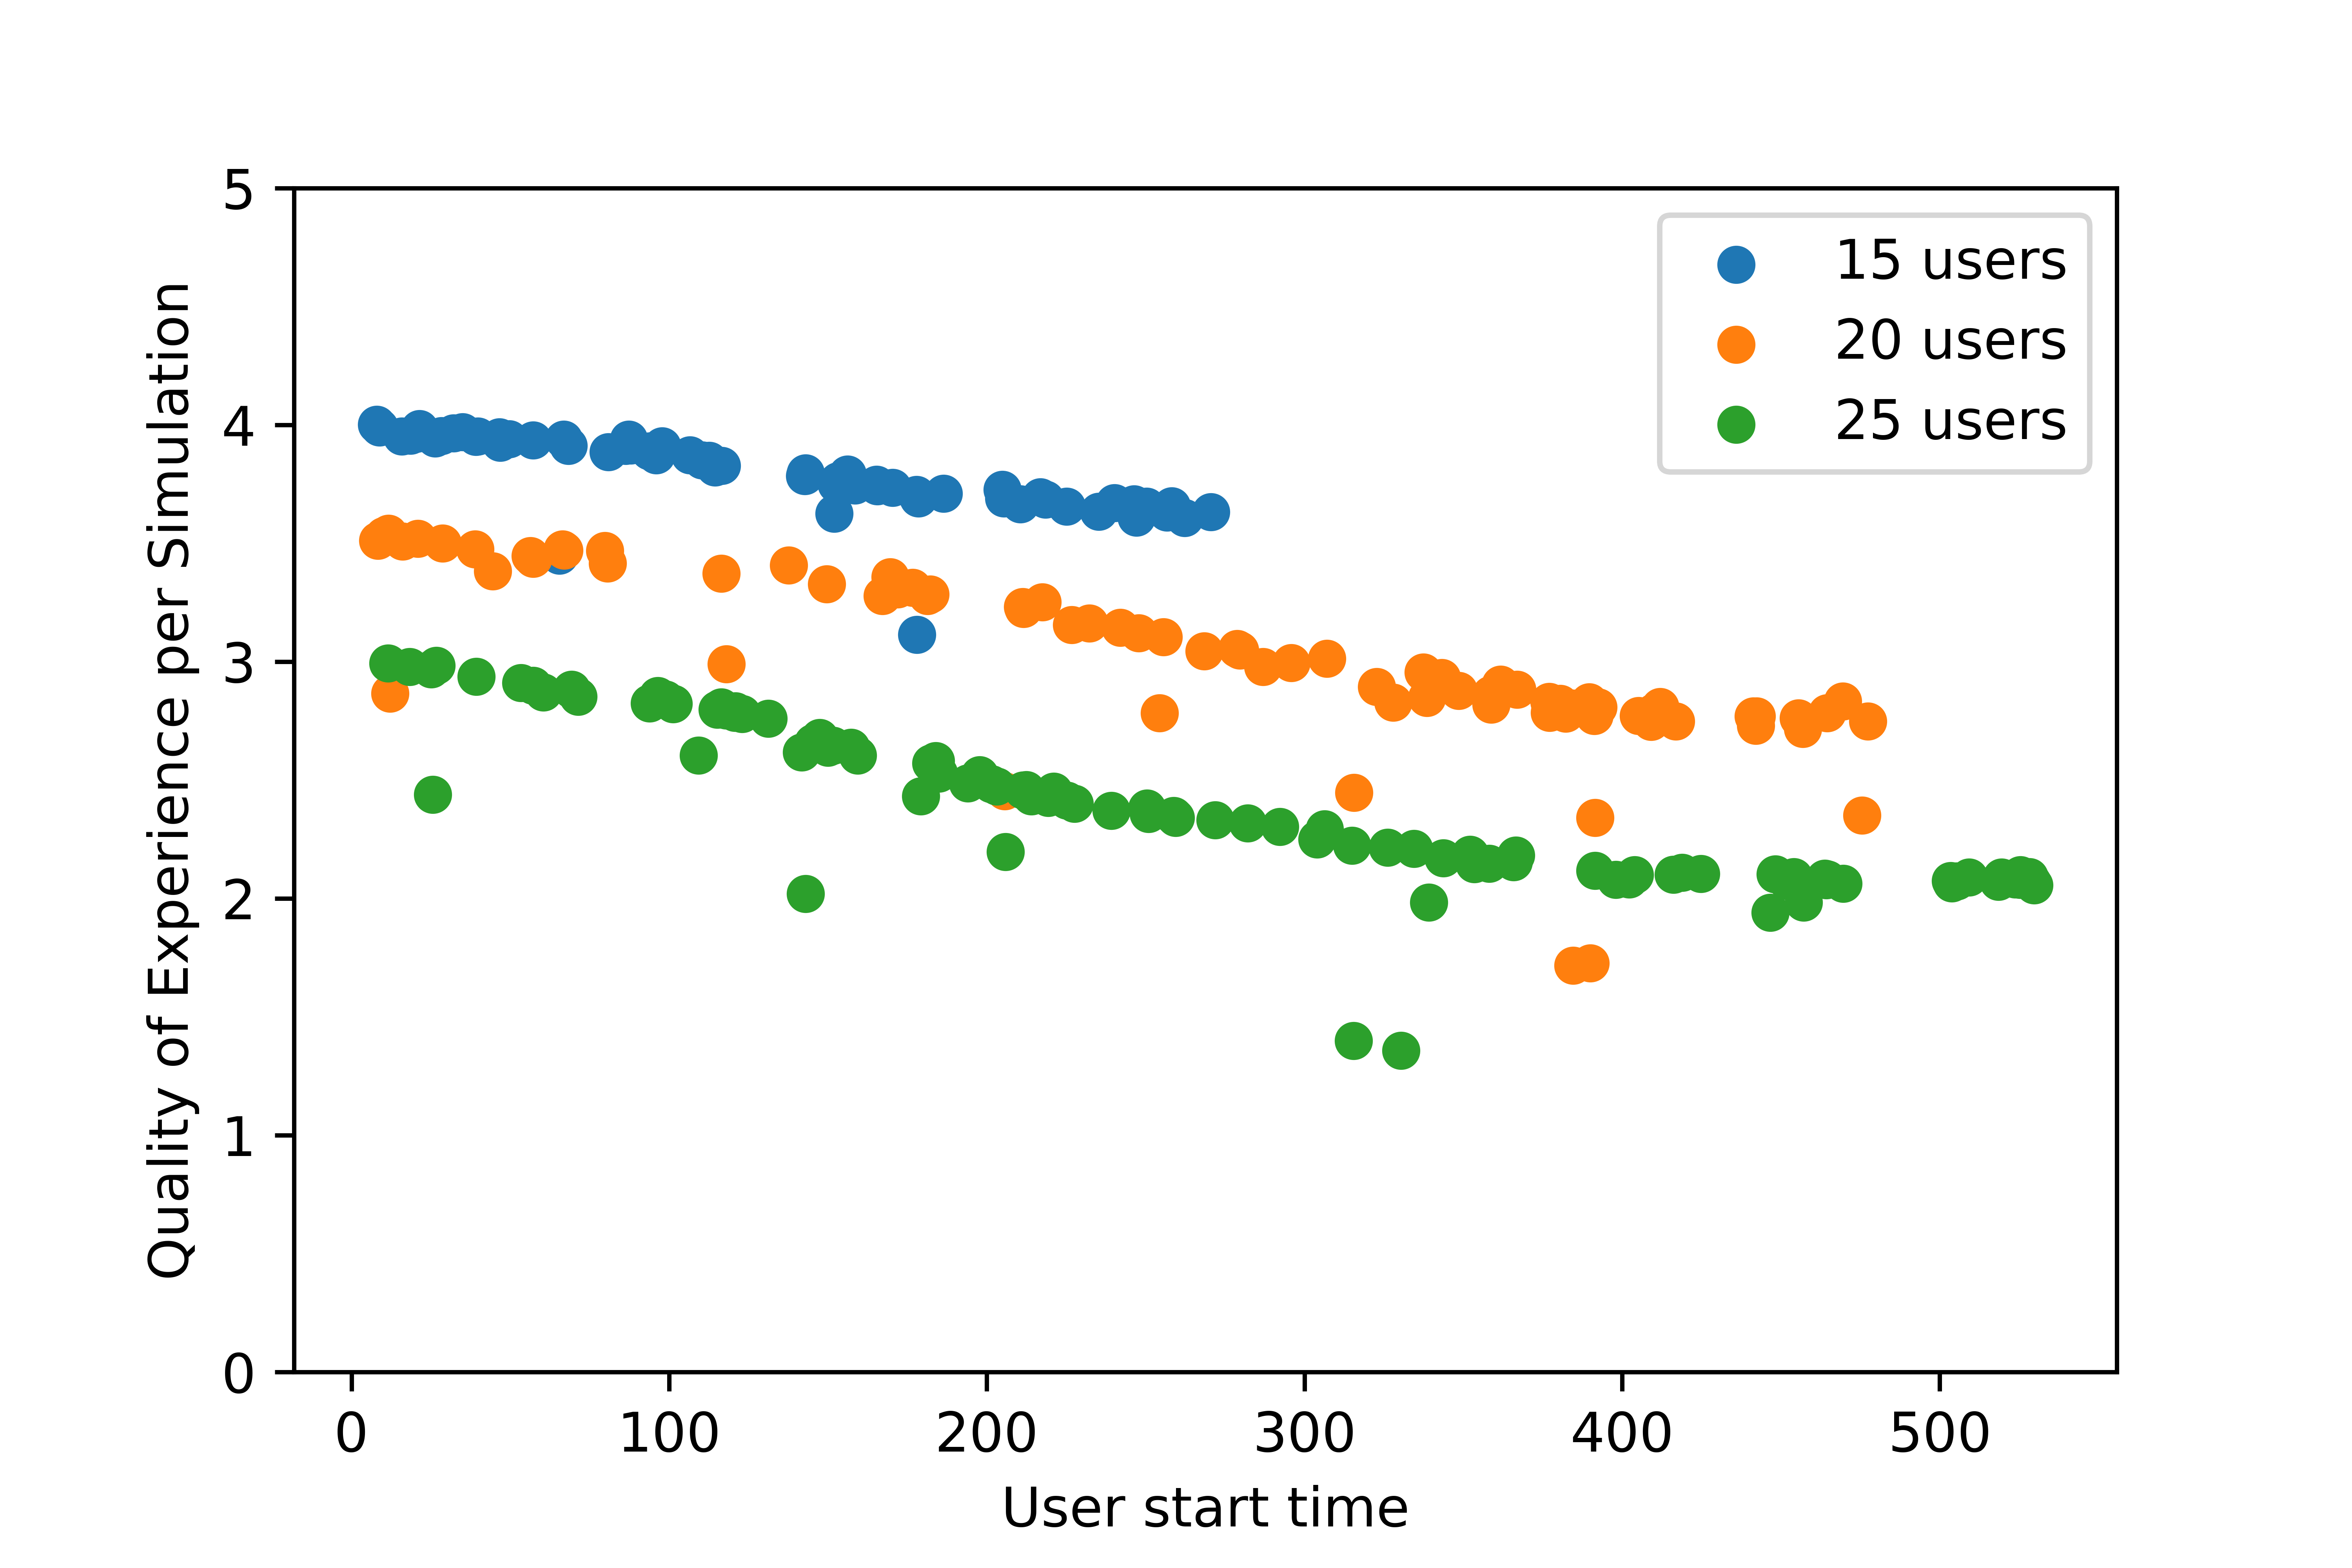
\includegraphics[width=0.45\linewidth]{images/QoECompare.png}
%     \label{fig:red-comparison-plot}
%     }
%     \subfigure[]{
%     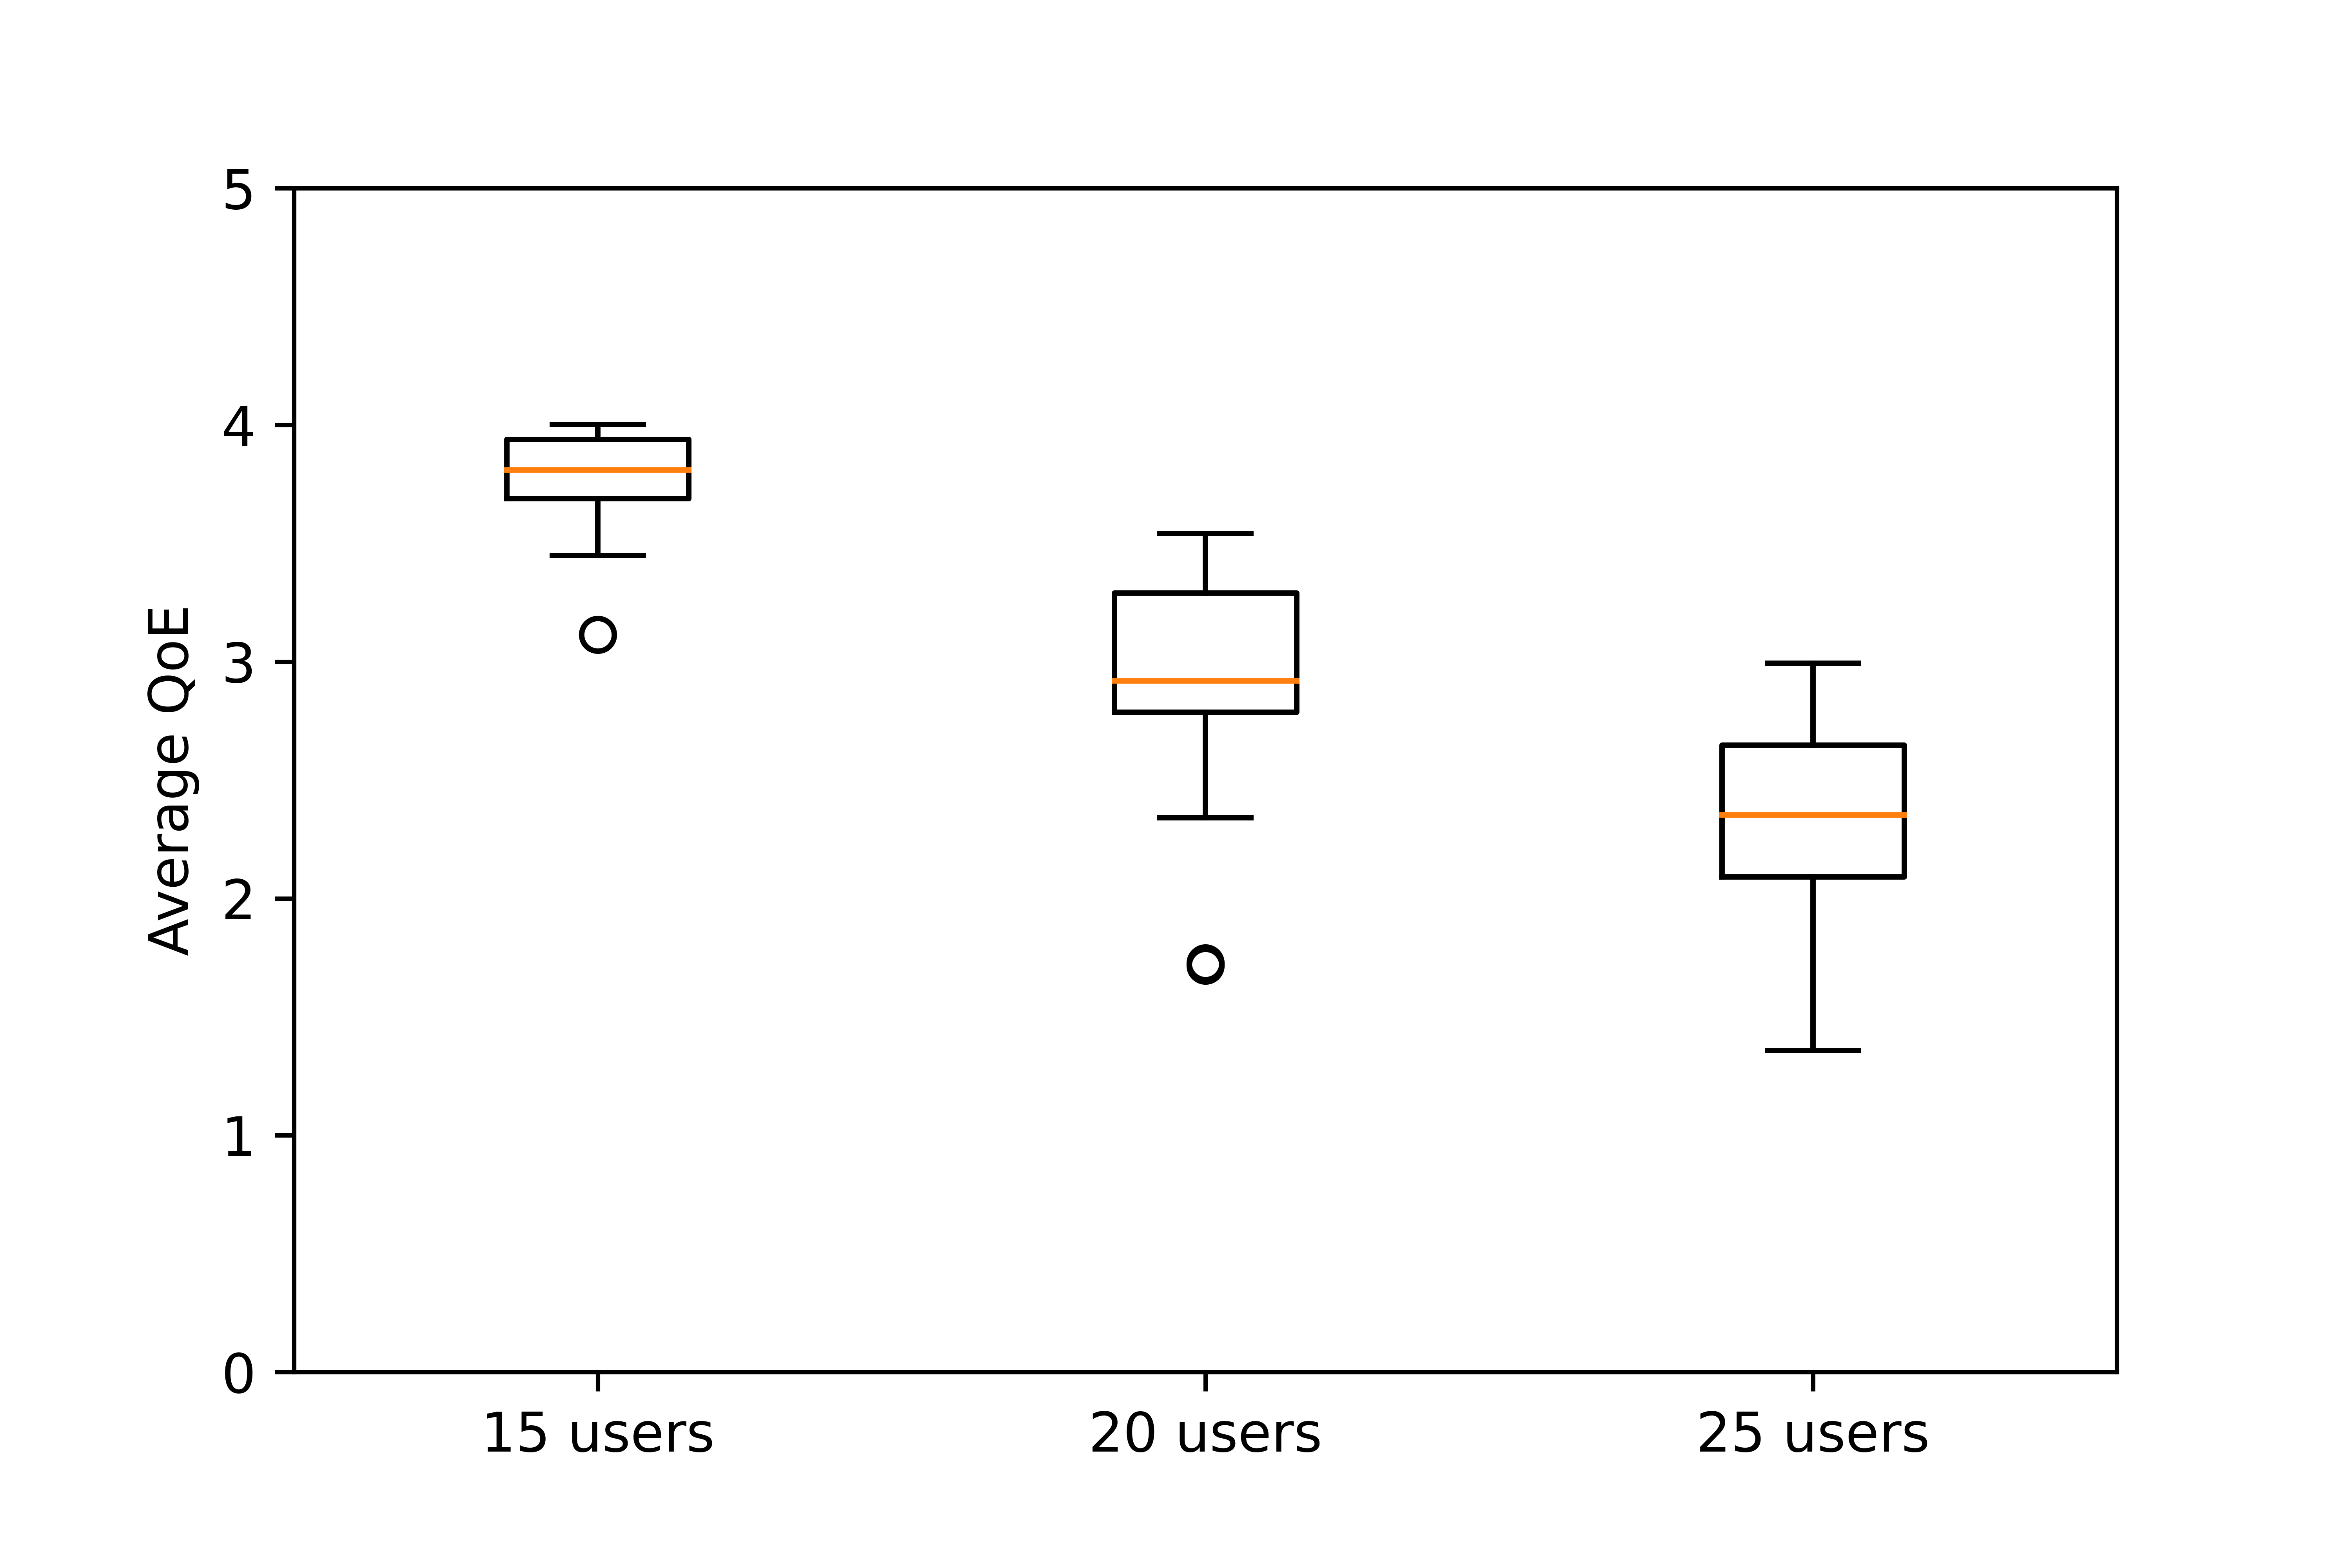
\includegraphics[width=0.45\linewidth]{images/QoEBoxplot.png}
%     \label{fig:red-comparison-boxplot}
%     }

%     \caption{Impact of system on the network performance. Distance \textit{d} between sensor node and antennas of 8m in a semi-NLOS scenario.}
%     \label{fig:comparison-rof-2}
% \end{figure*}

\begin{figure*}
    \centering
    \subfigure[]{
    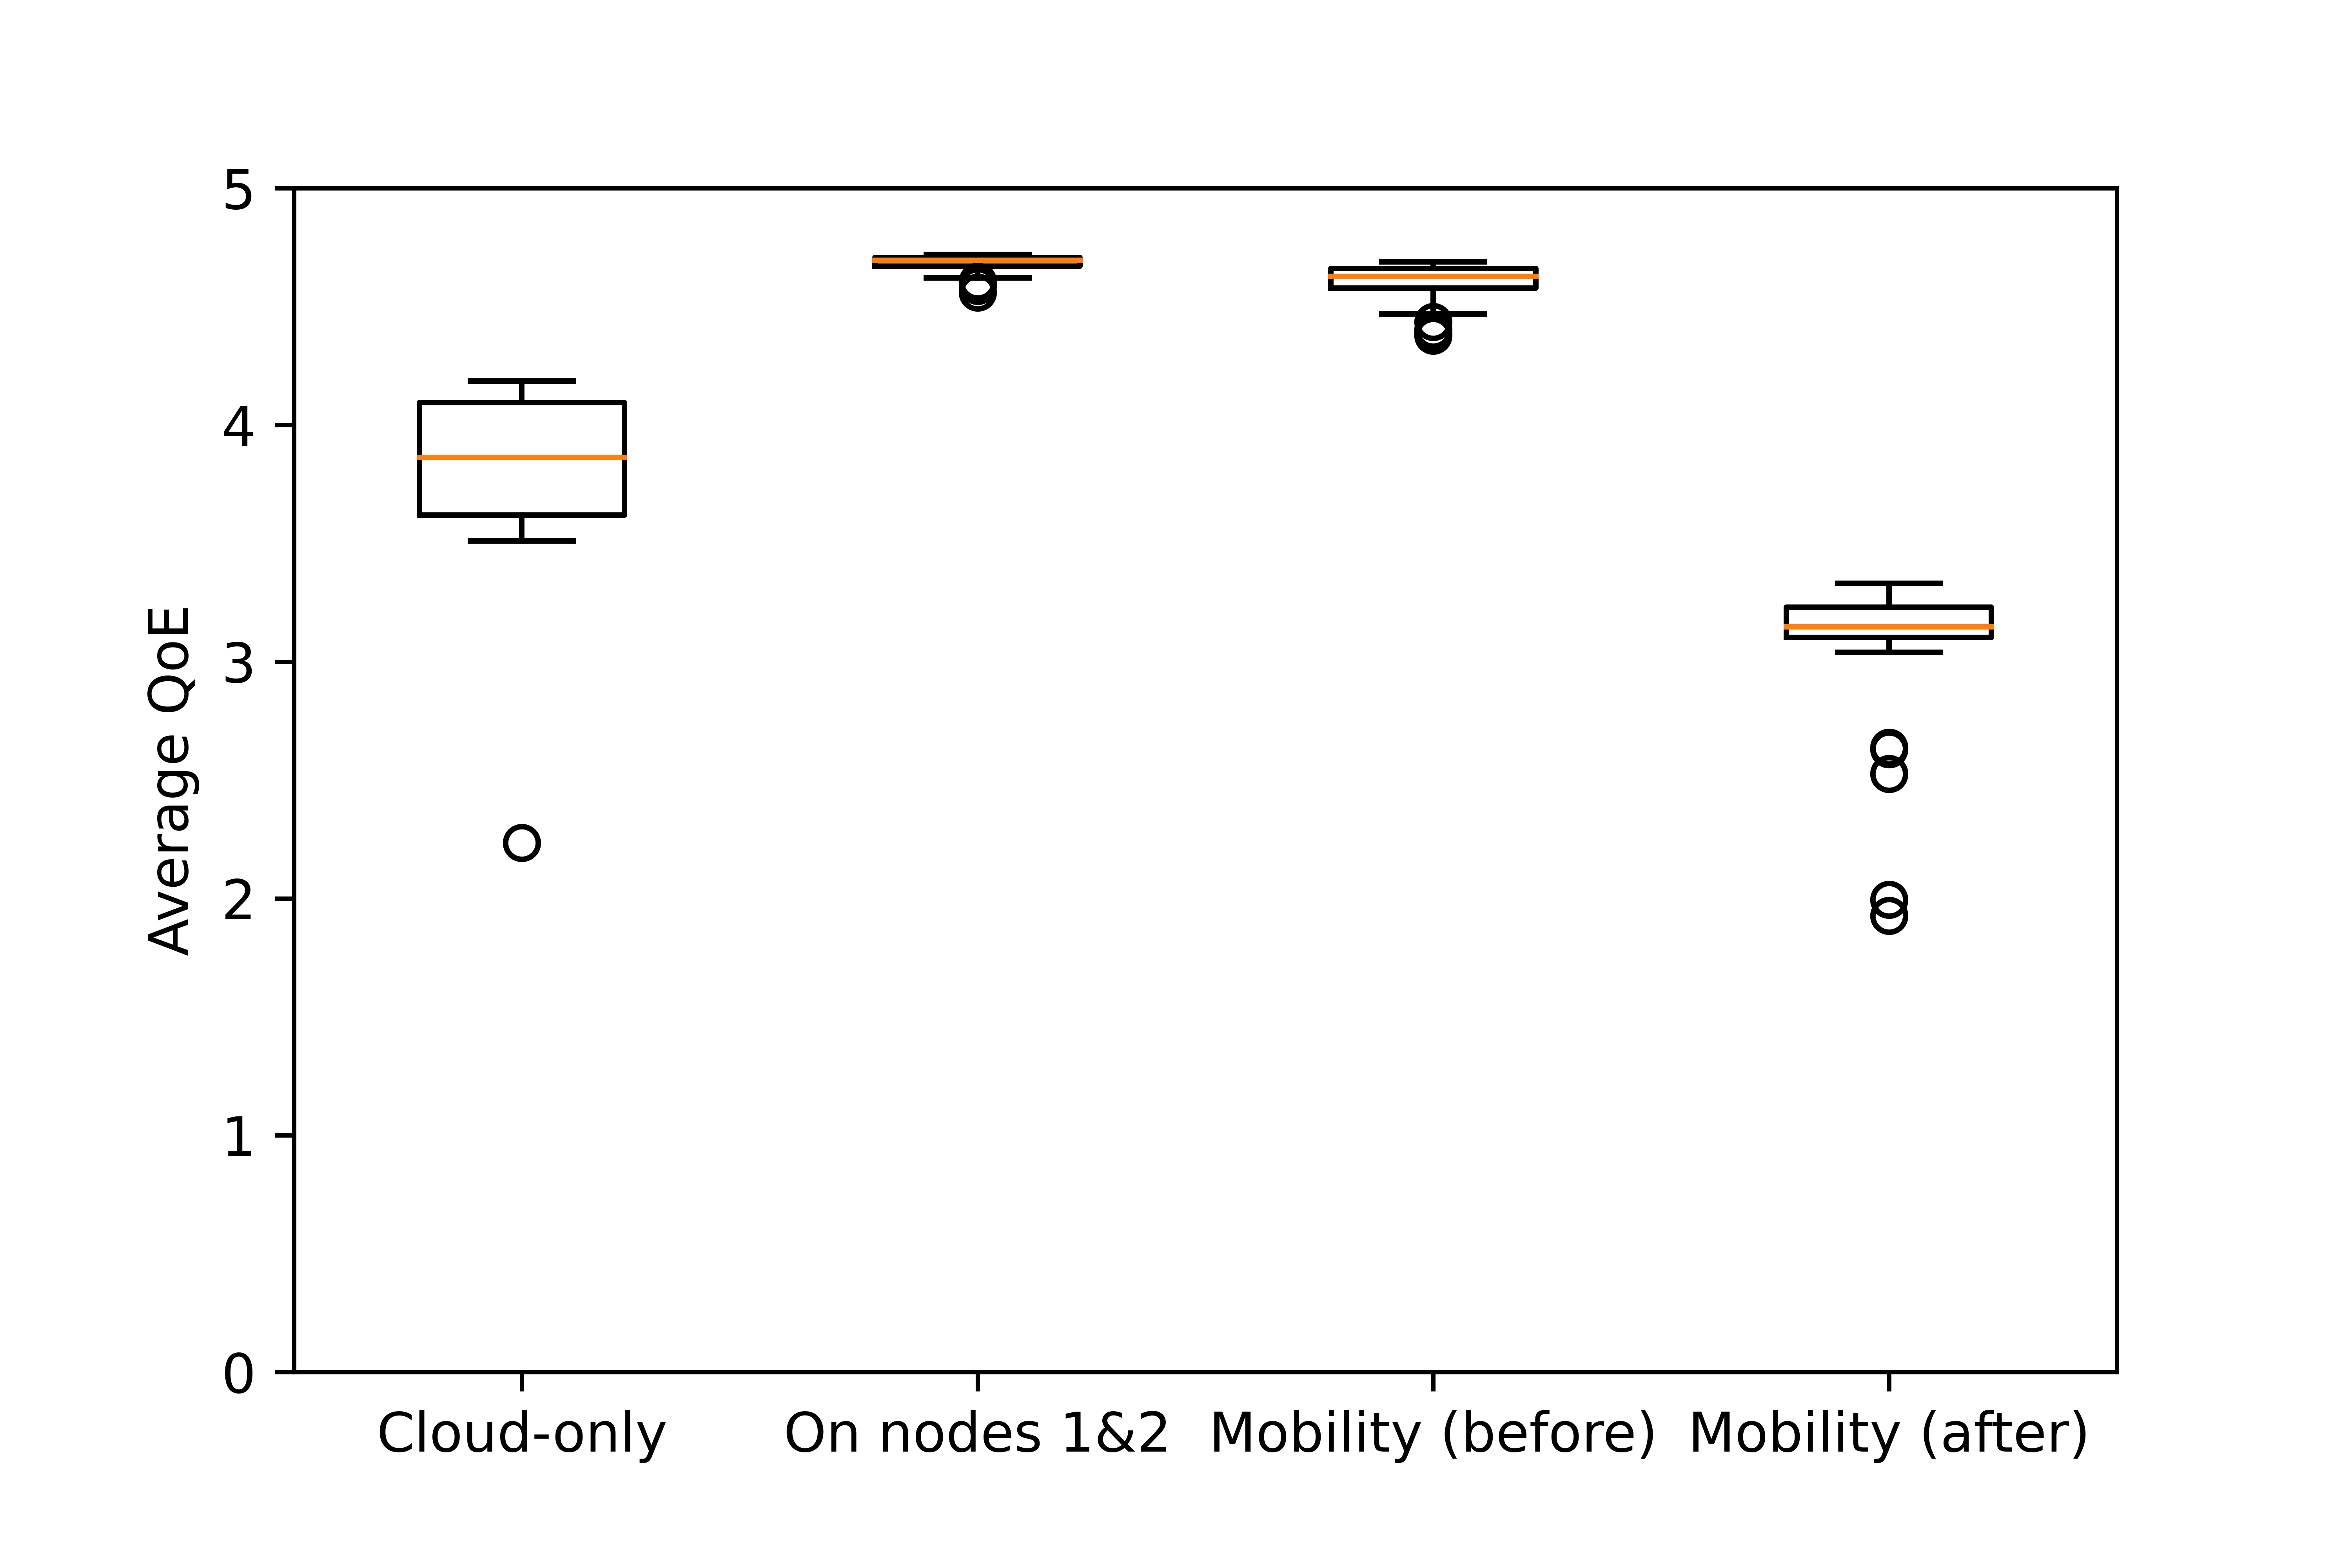
\includegraphics[width=0.31\linewidth]{images/QoEBoxplot-15u.png}
    \label{fig:red-comparison-plot}
    }
    \subfigure[]{
    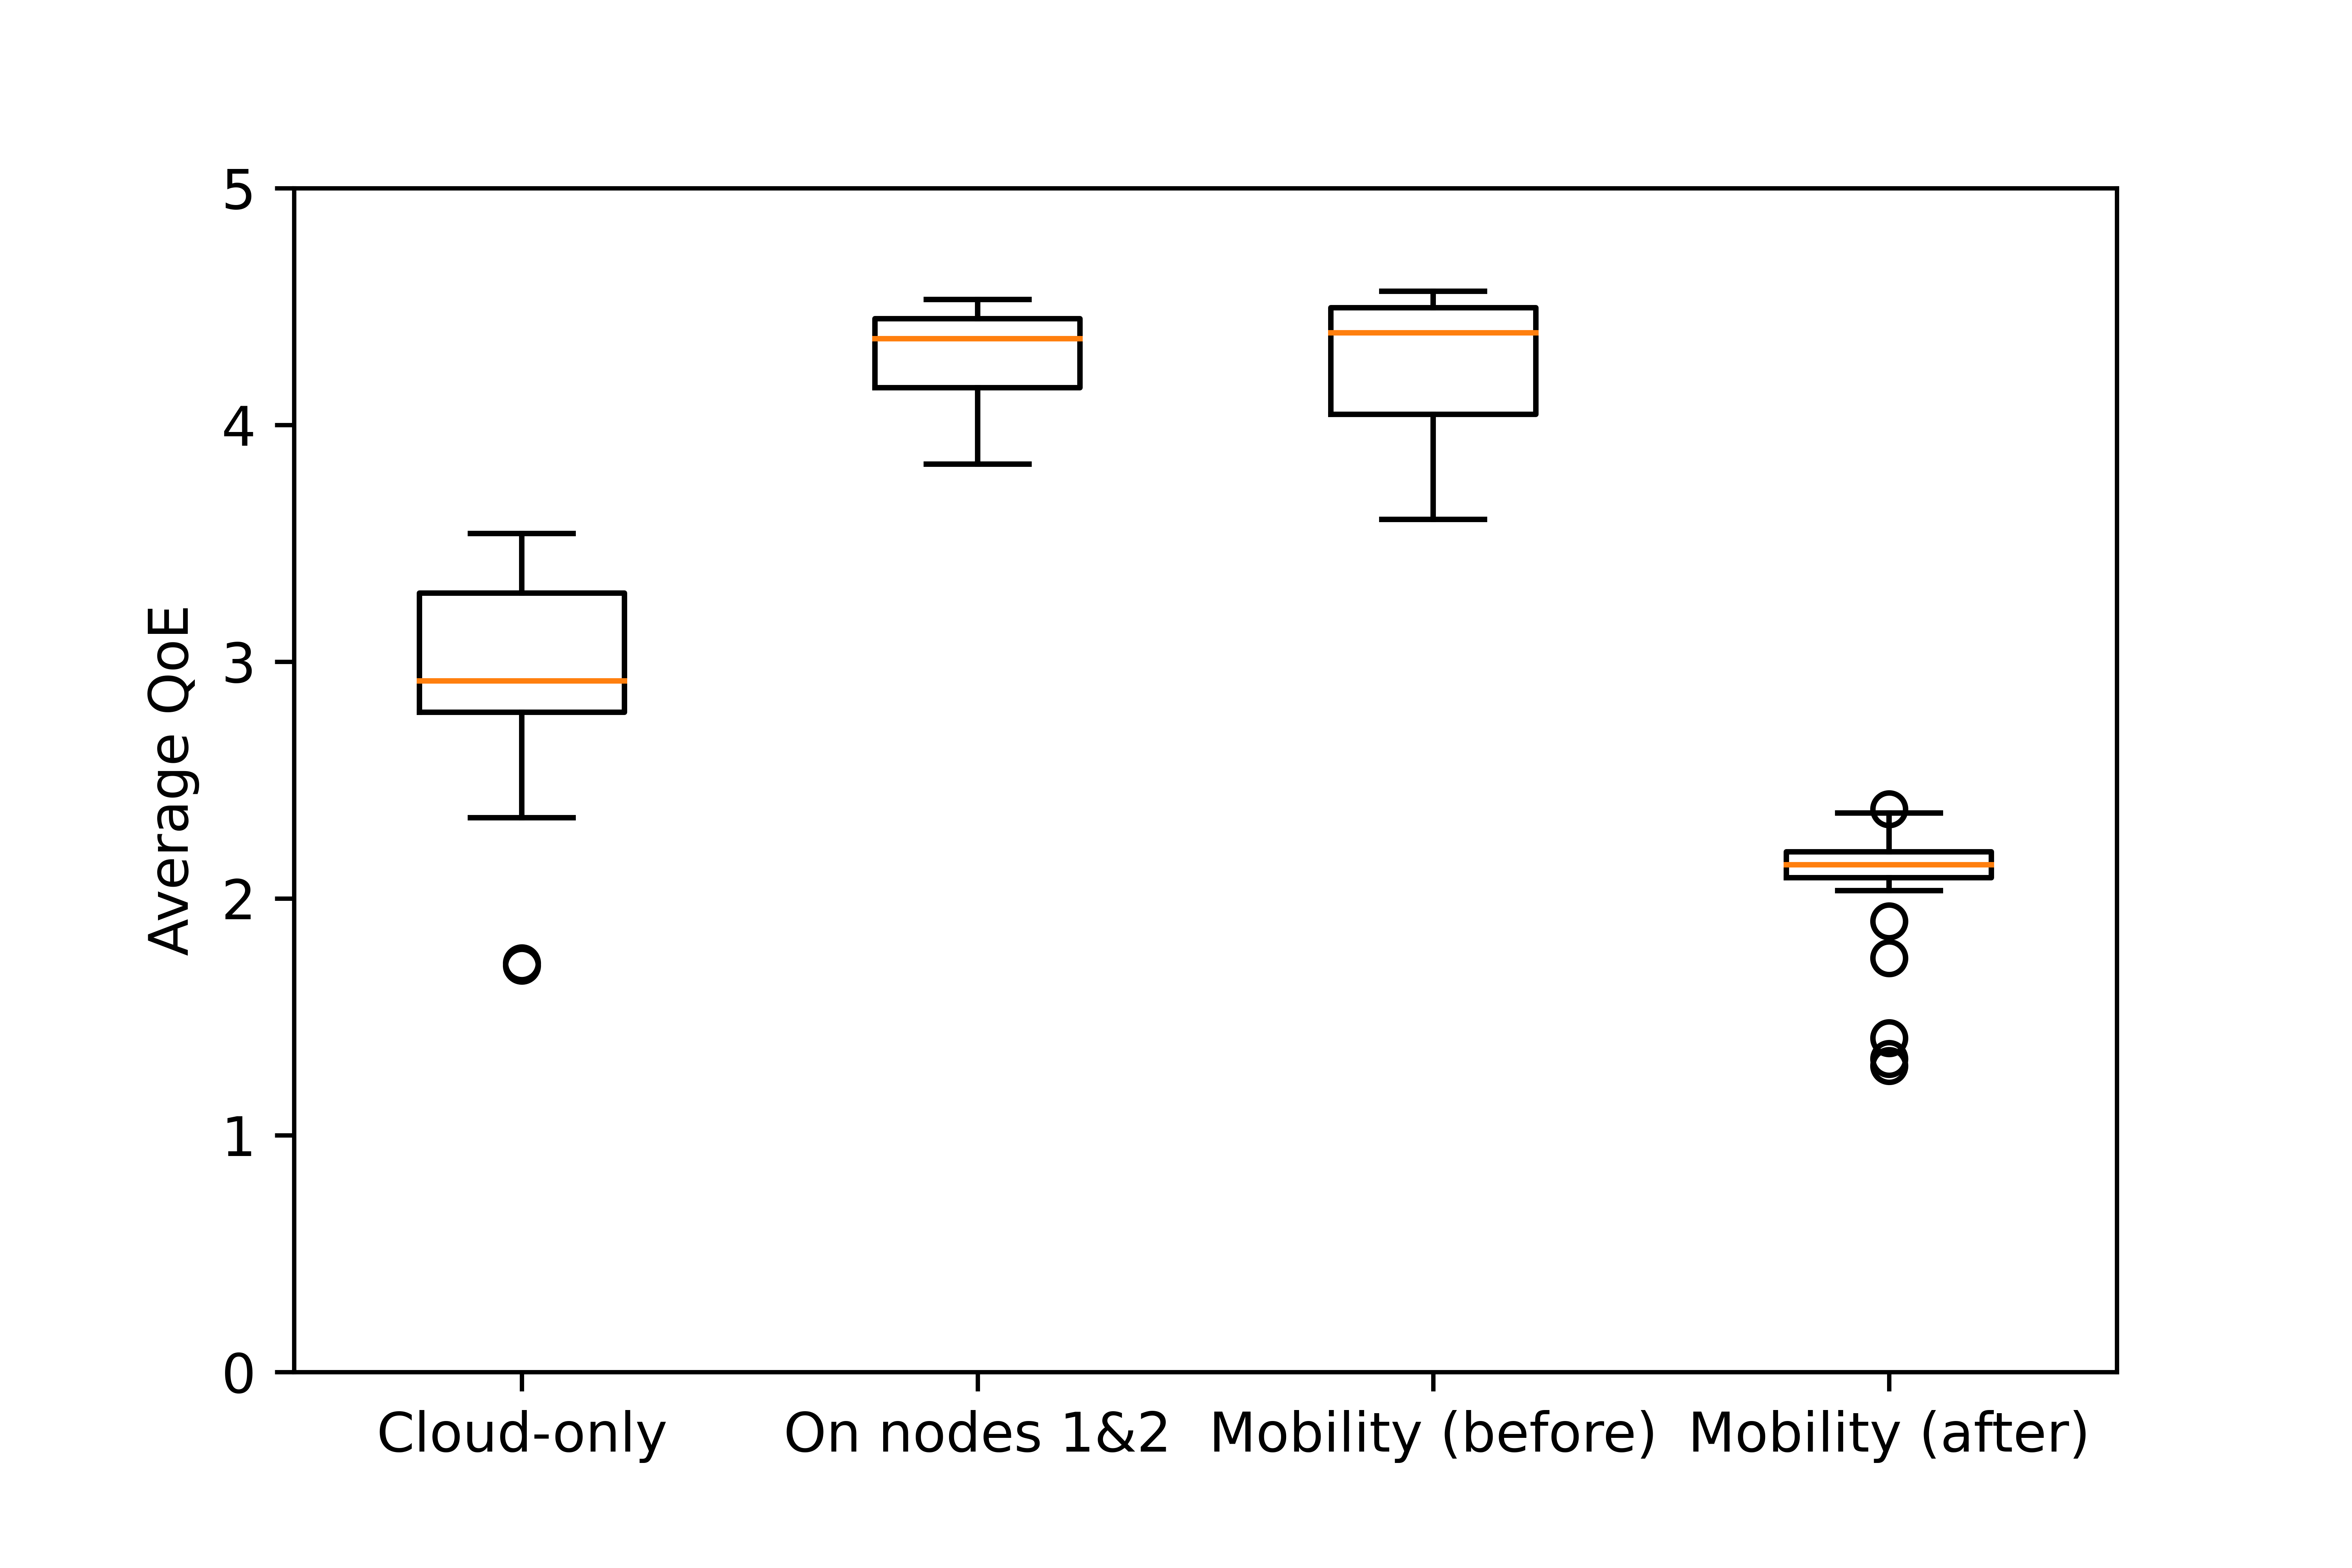
\includegraphics[width=0.31\linewidth]{images/QoEBoxplot-20u.png}
    \label{fig:co-comparison-boxplot}
    }
    \subfigure[]{
    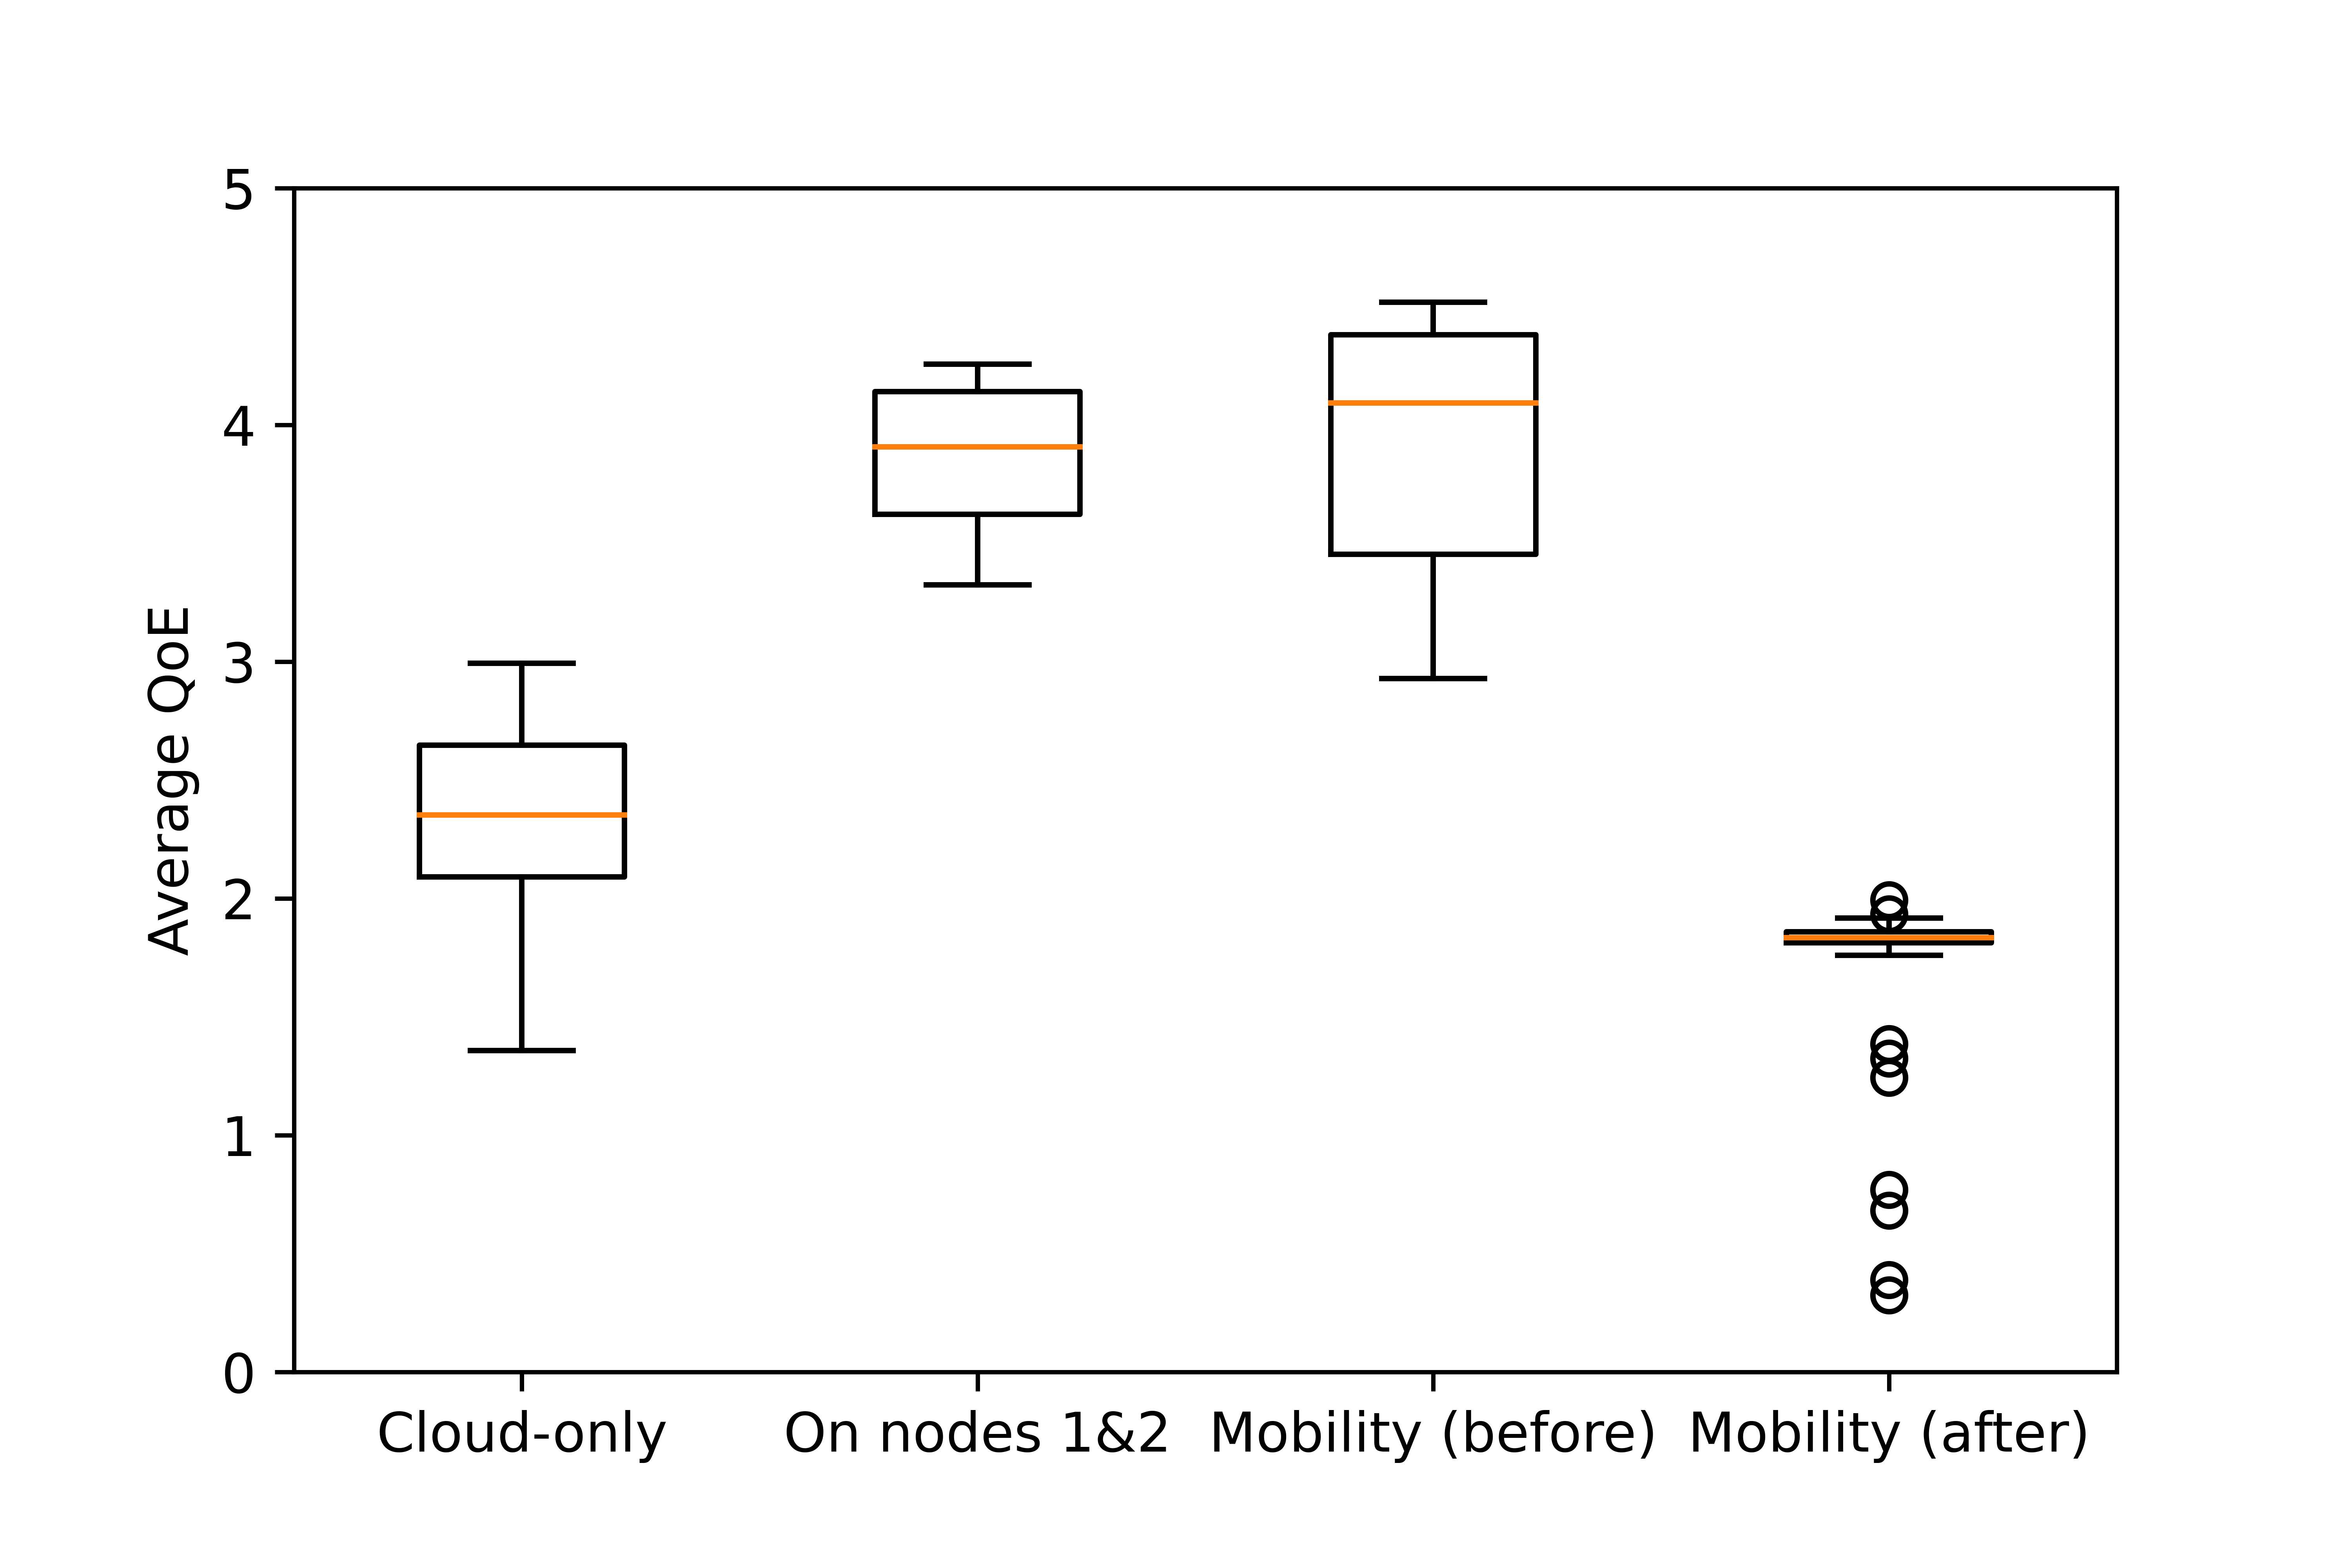
\includegraphics[width=0.31\linewidth]{images/QoEBoxplot-25u.png}
    \label{fig:red-comparison-plot}
    }
    
    \caption{Average QoE results for scenarios with 15, 20 and 25 users per AP.}
    \label{fig:comparison-rof-2}
\end{figure*}


\begin{figure*}
    \centering
    \subfigure[]{
    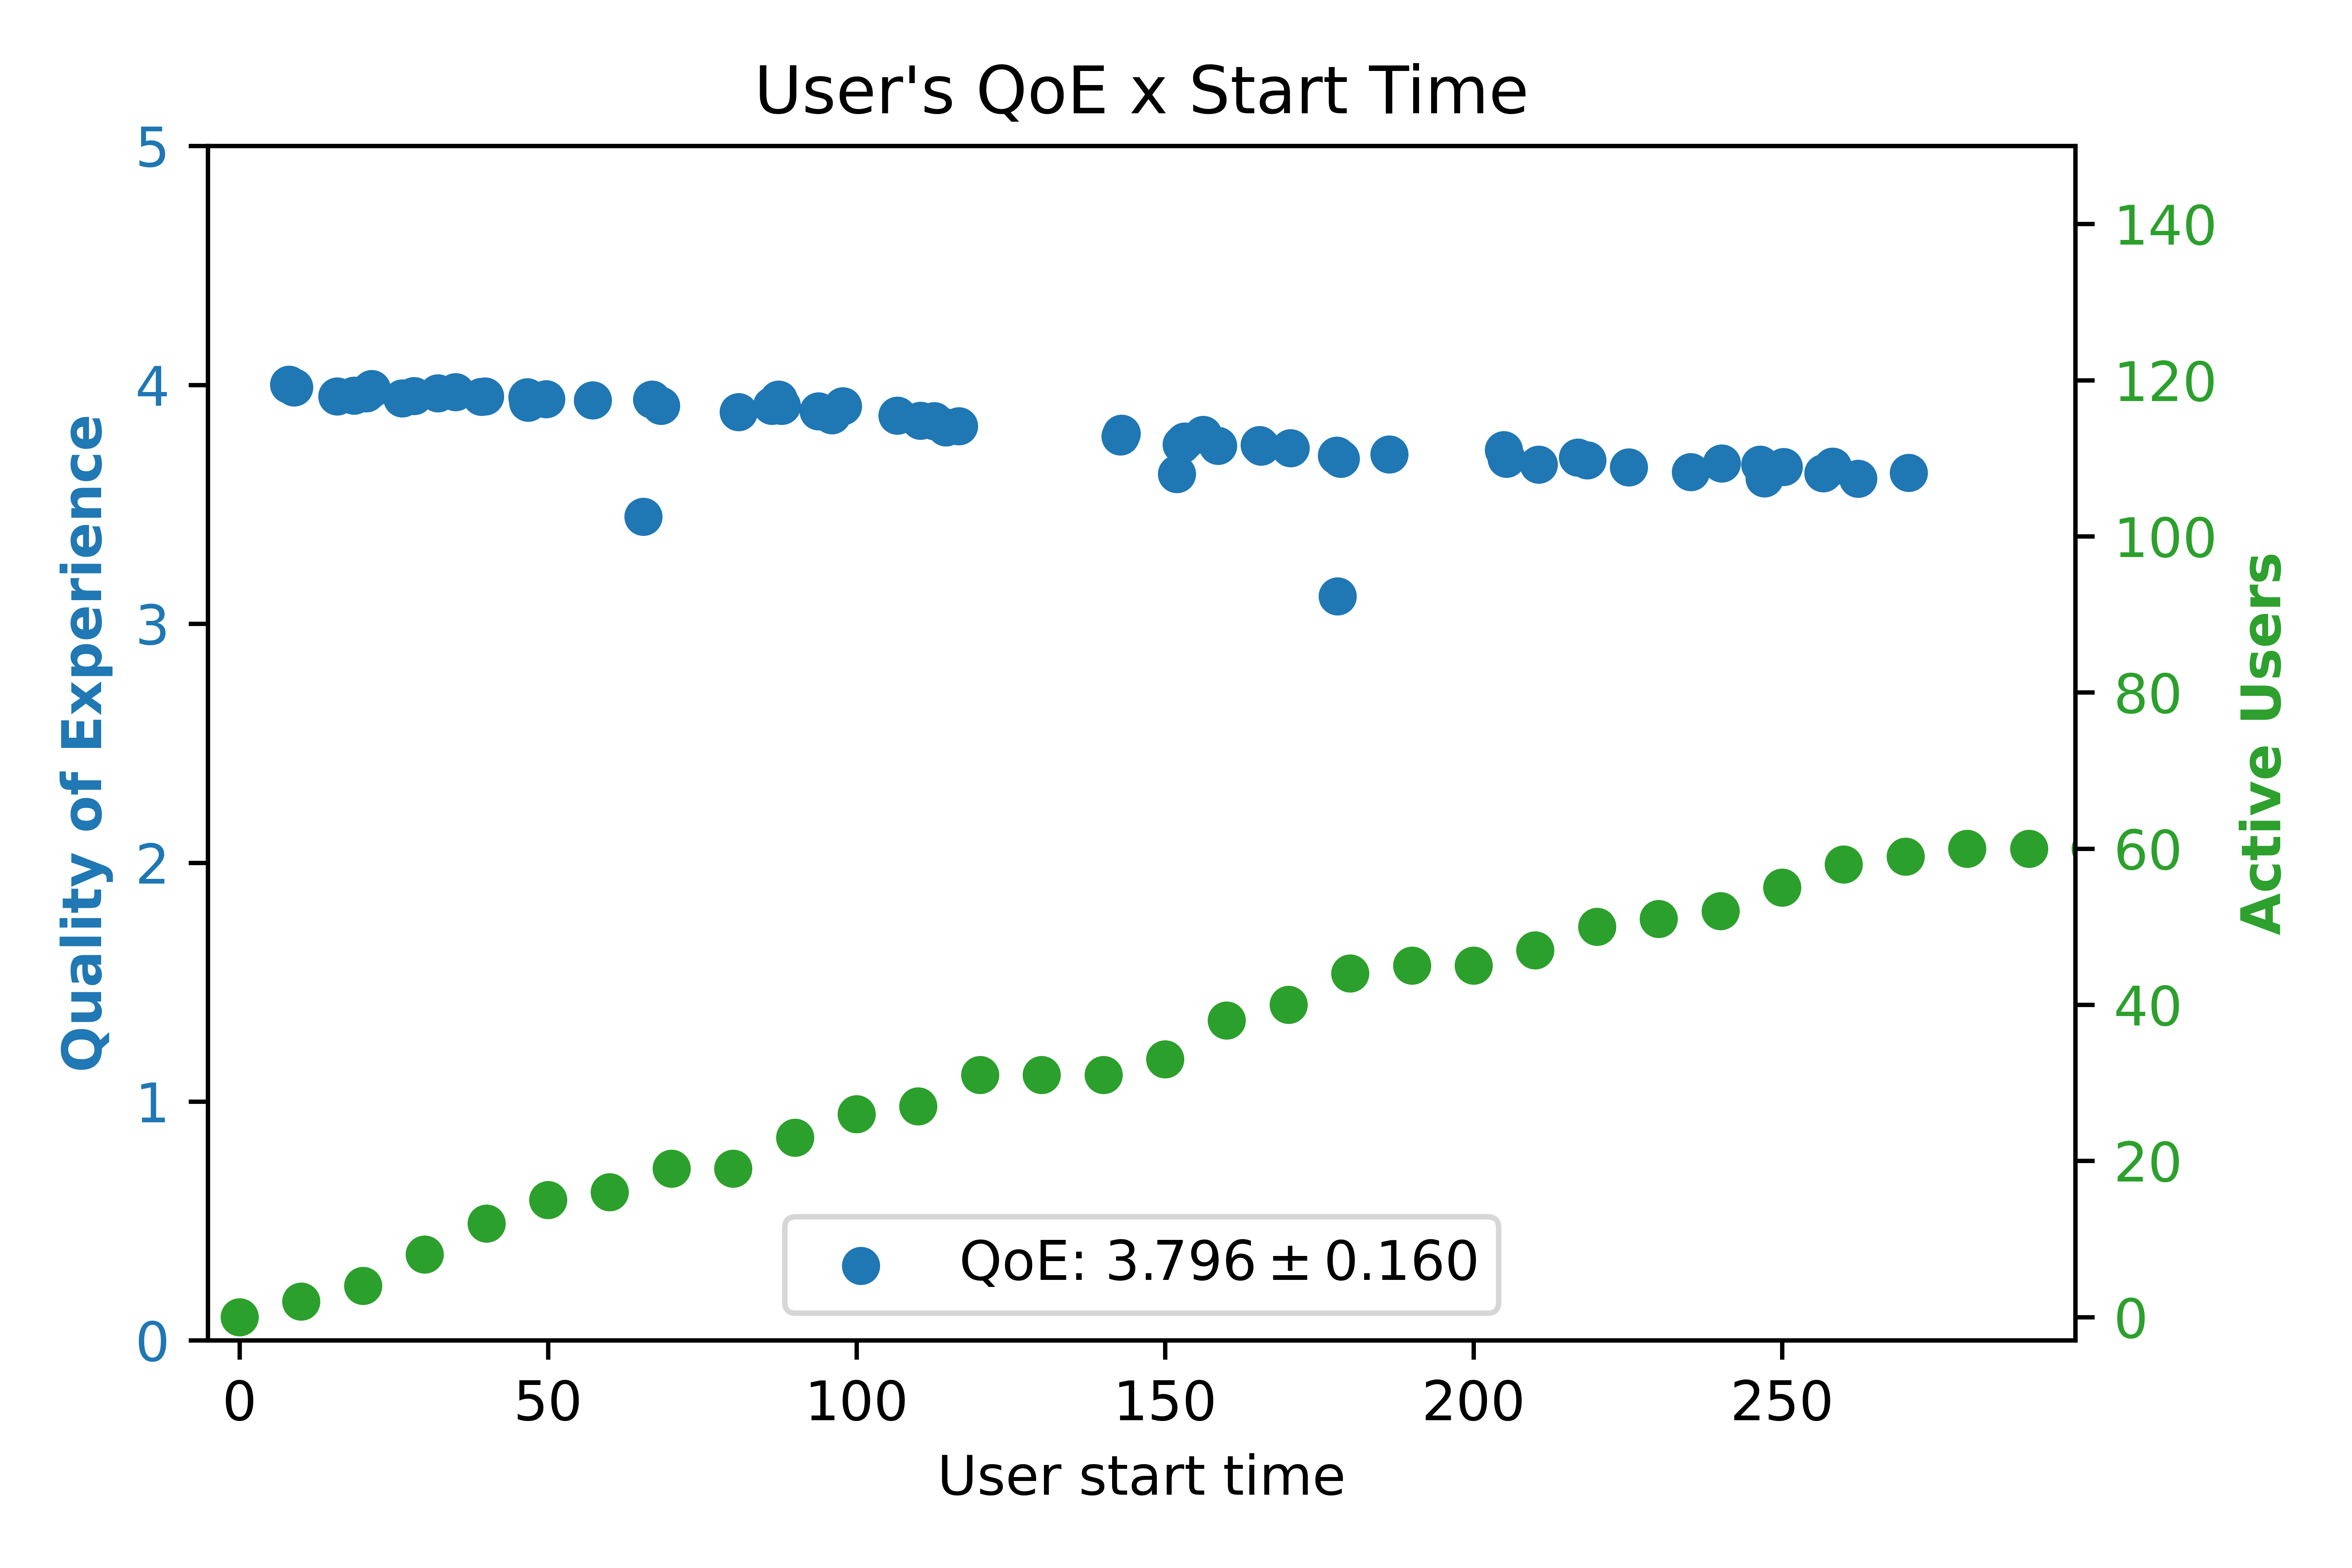
\includegraphics[width=0.31\linewidth]{images/cloud_QoExStartTime15.png}
    \label{fig:rssi-comparison-2}
    }
    \subfigure[]{
    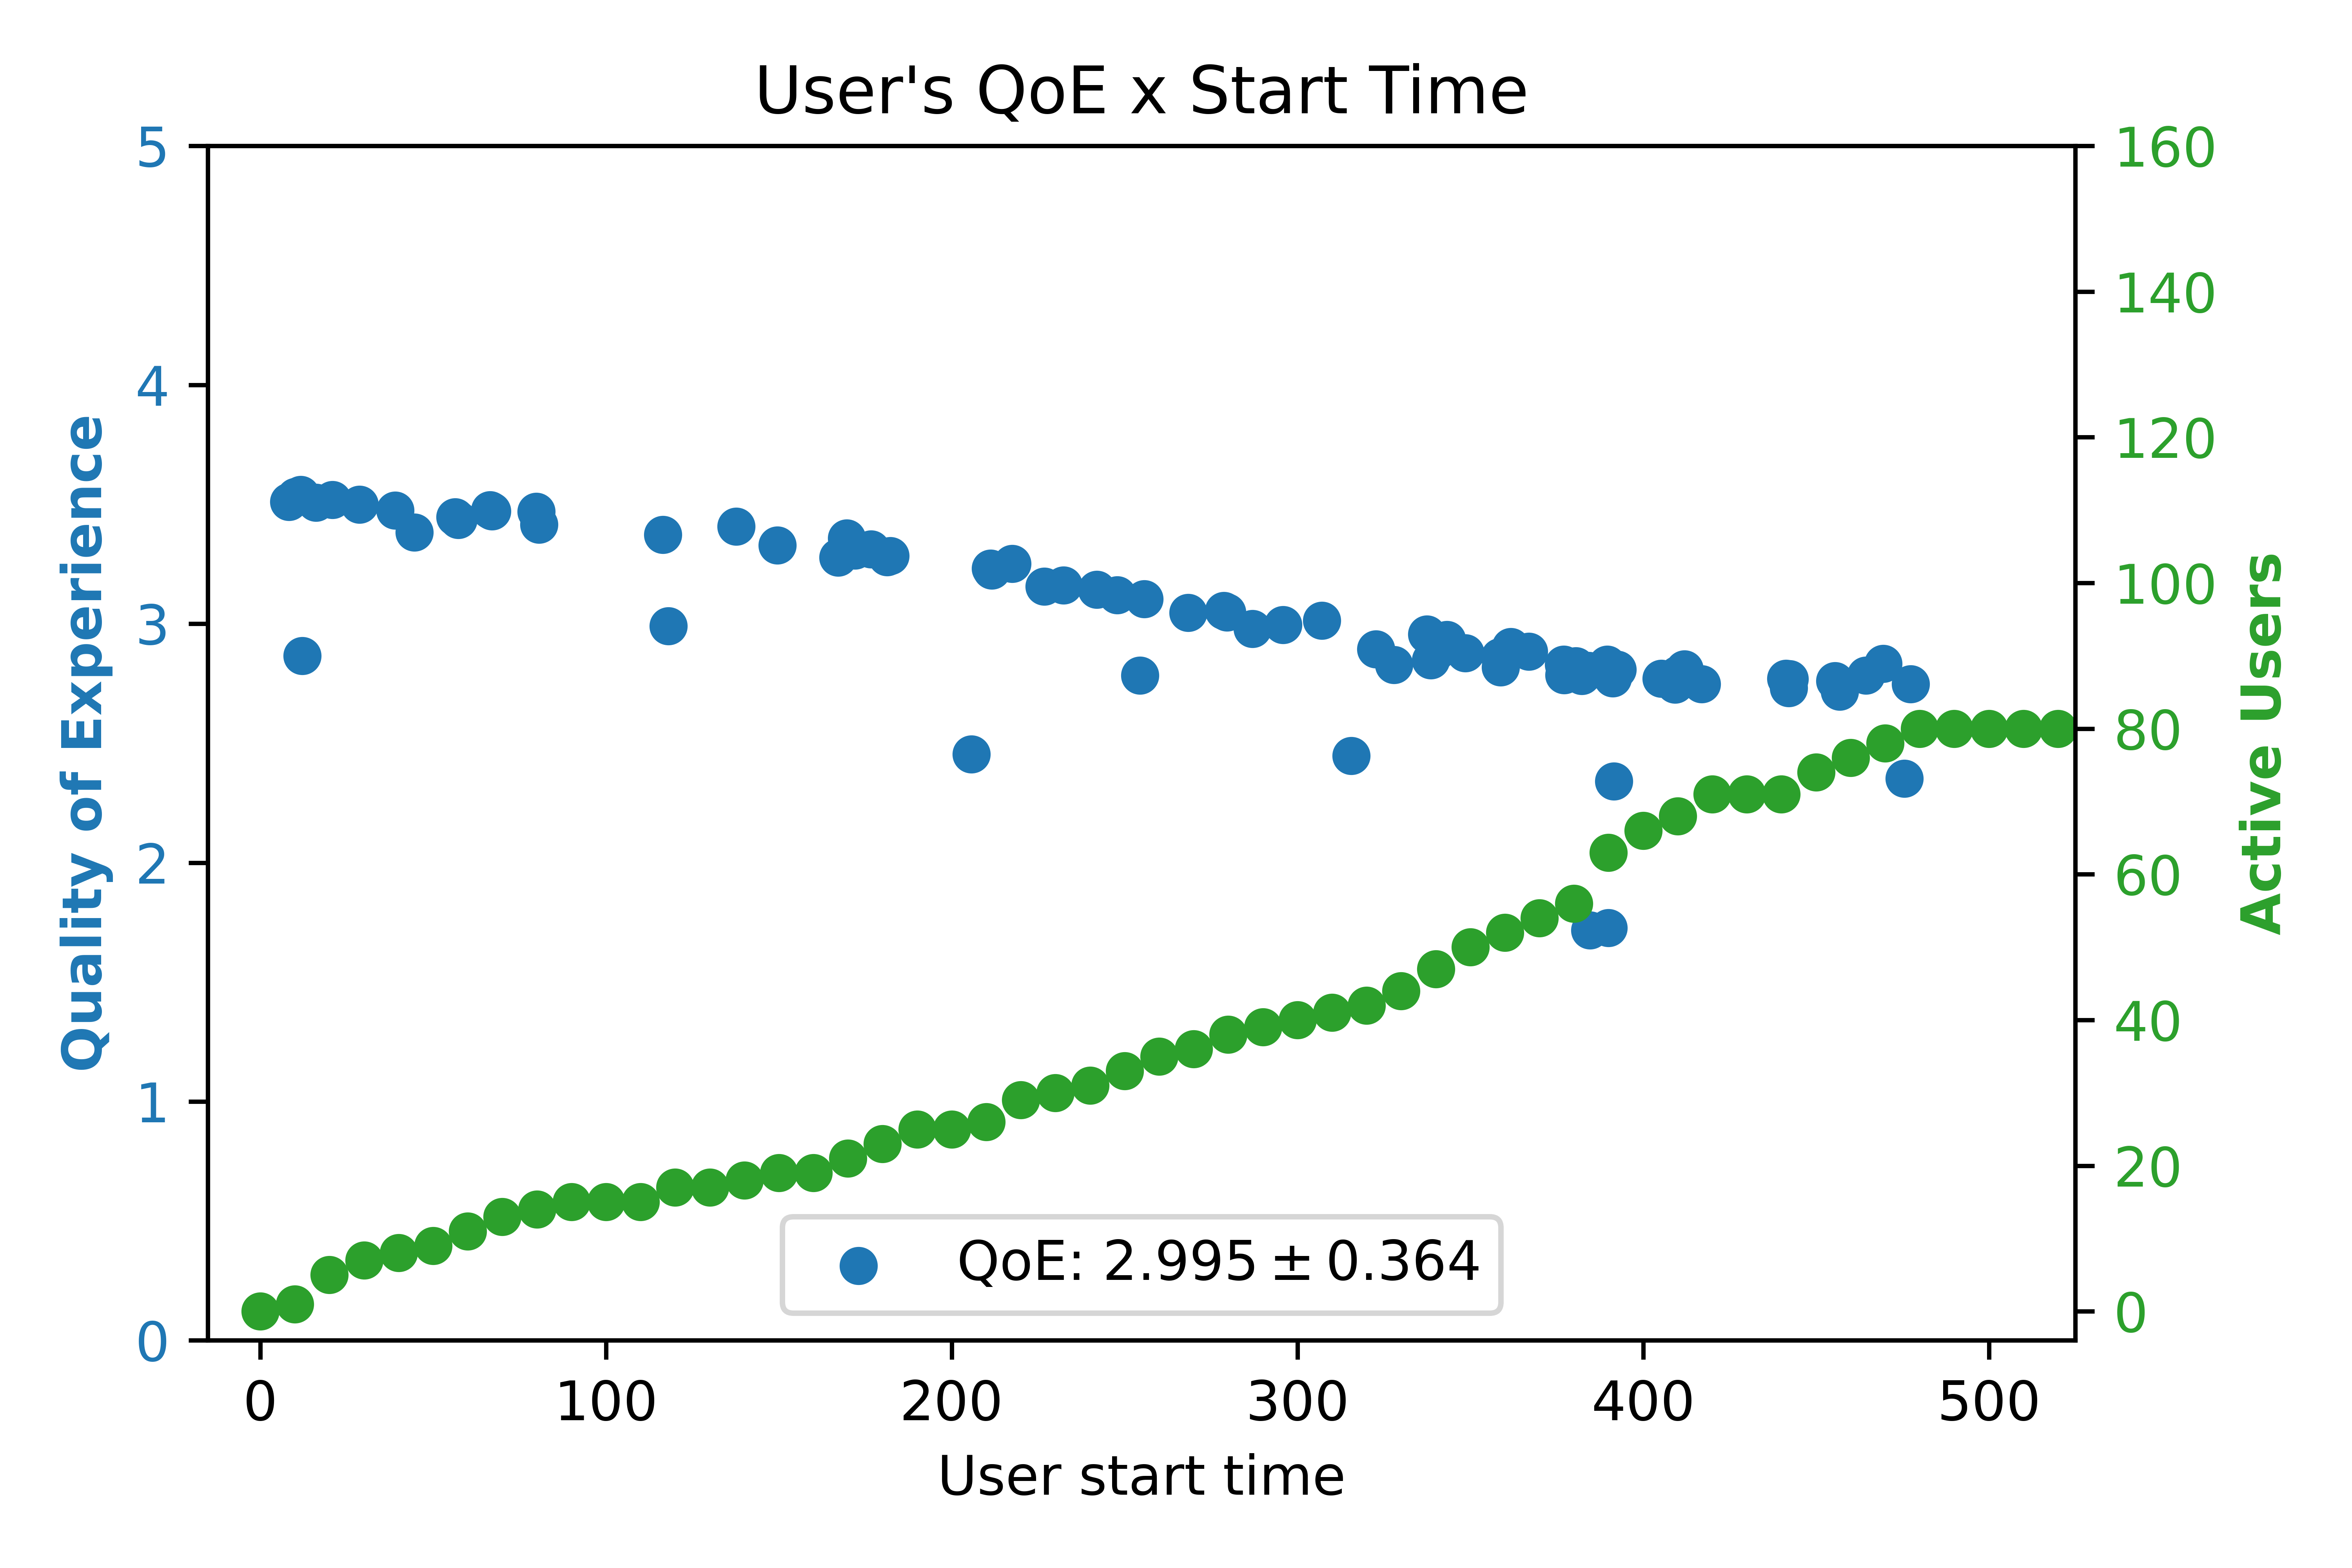
\includegraphics[width=0.31\linewidth]{images/cloud_QoExStartTime20.png}
    \label{fig:plr-comparison-2}
    }
    \subfigure[]{
    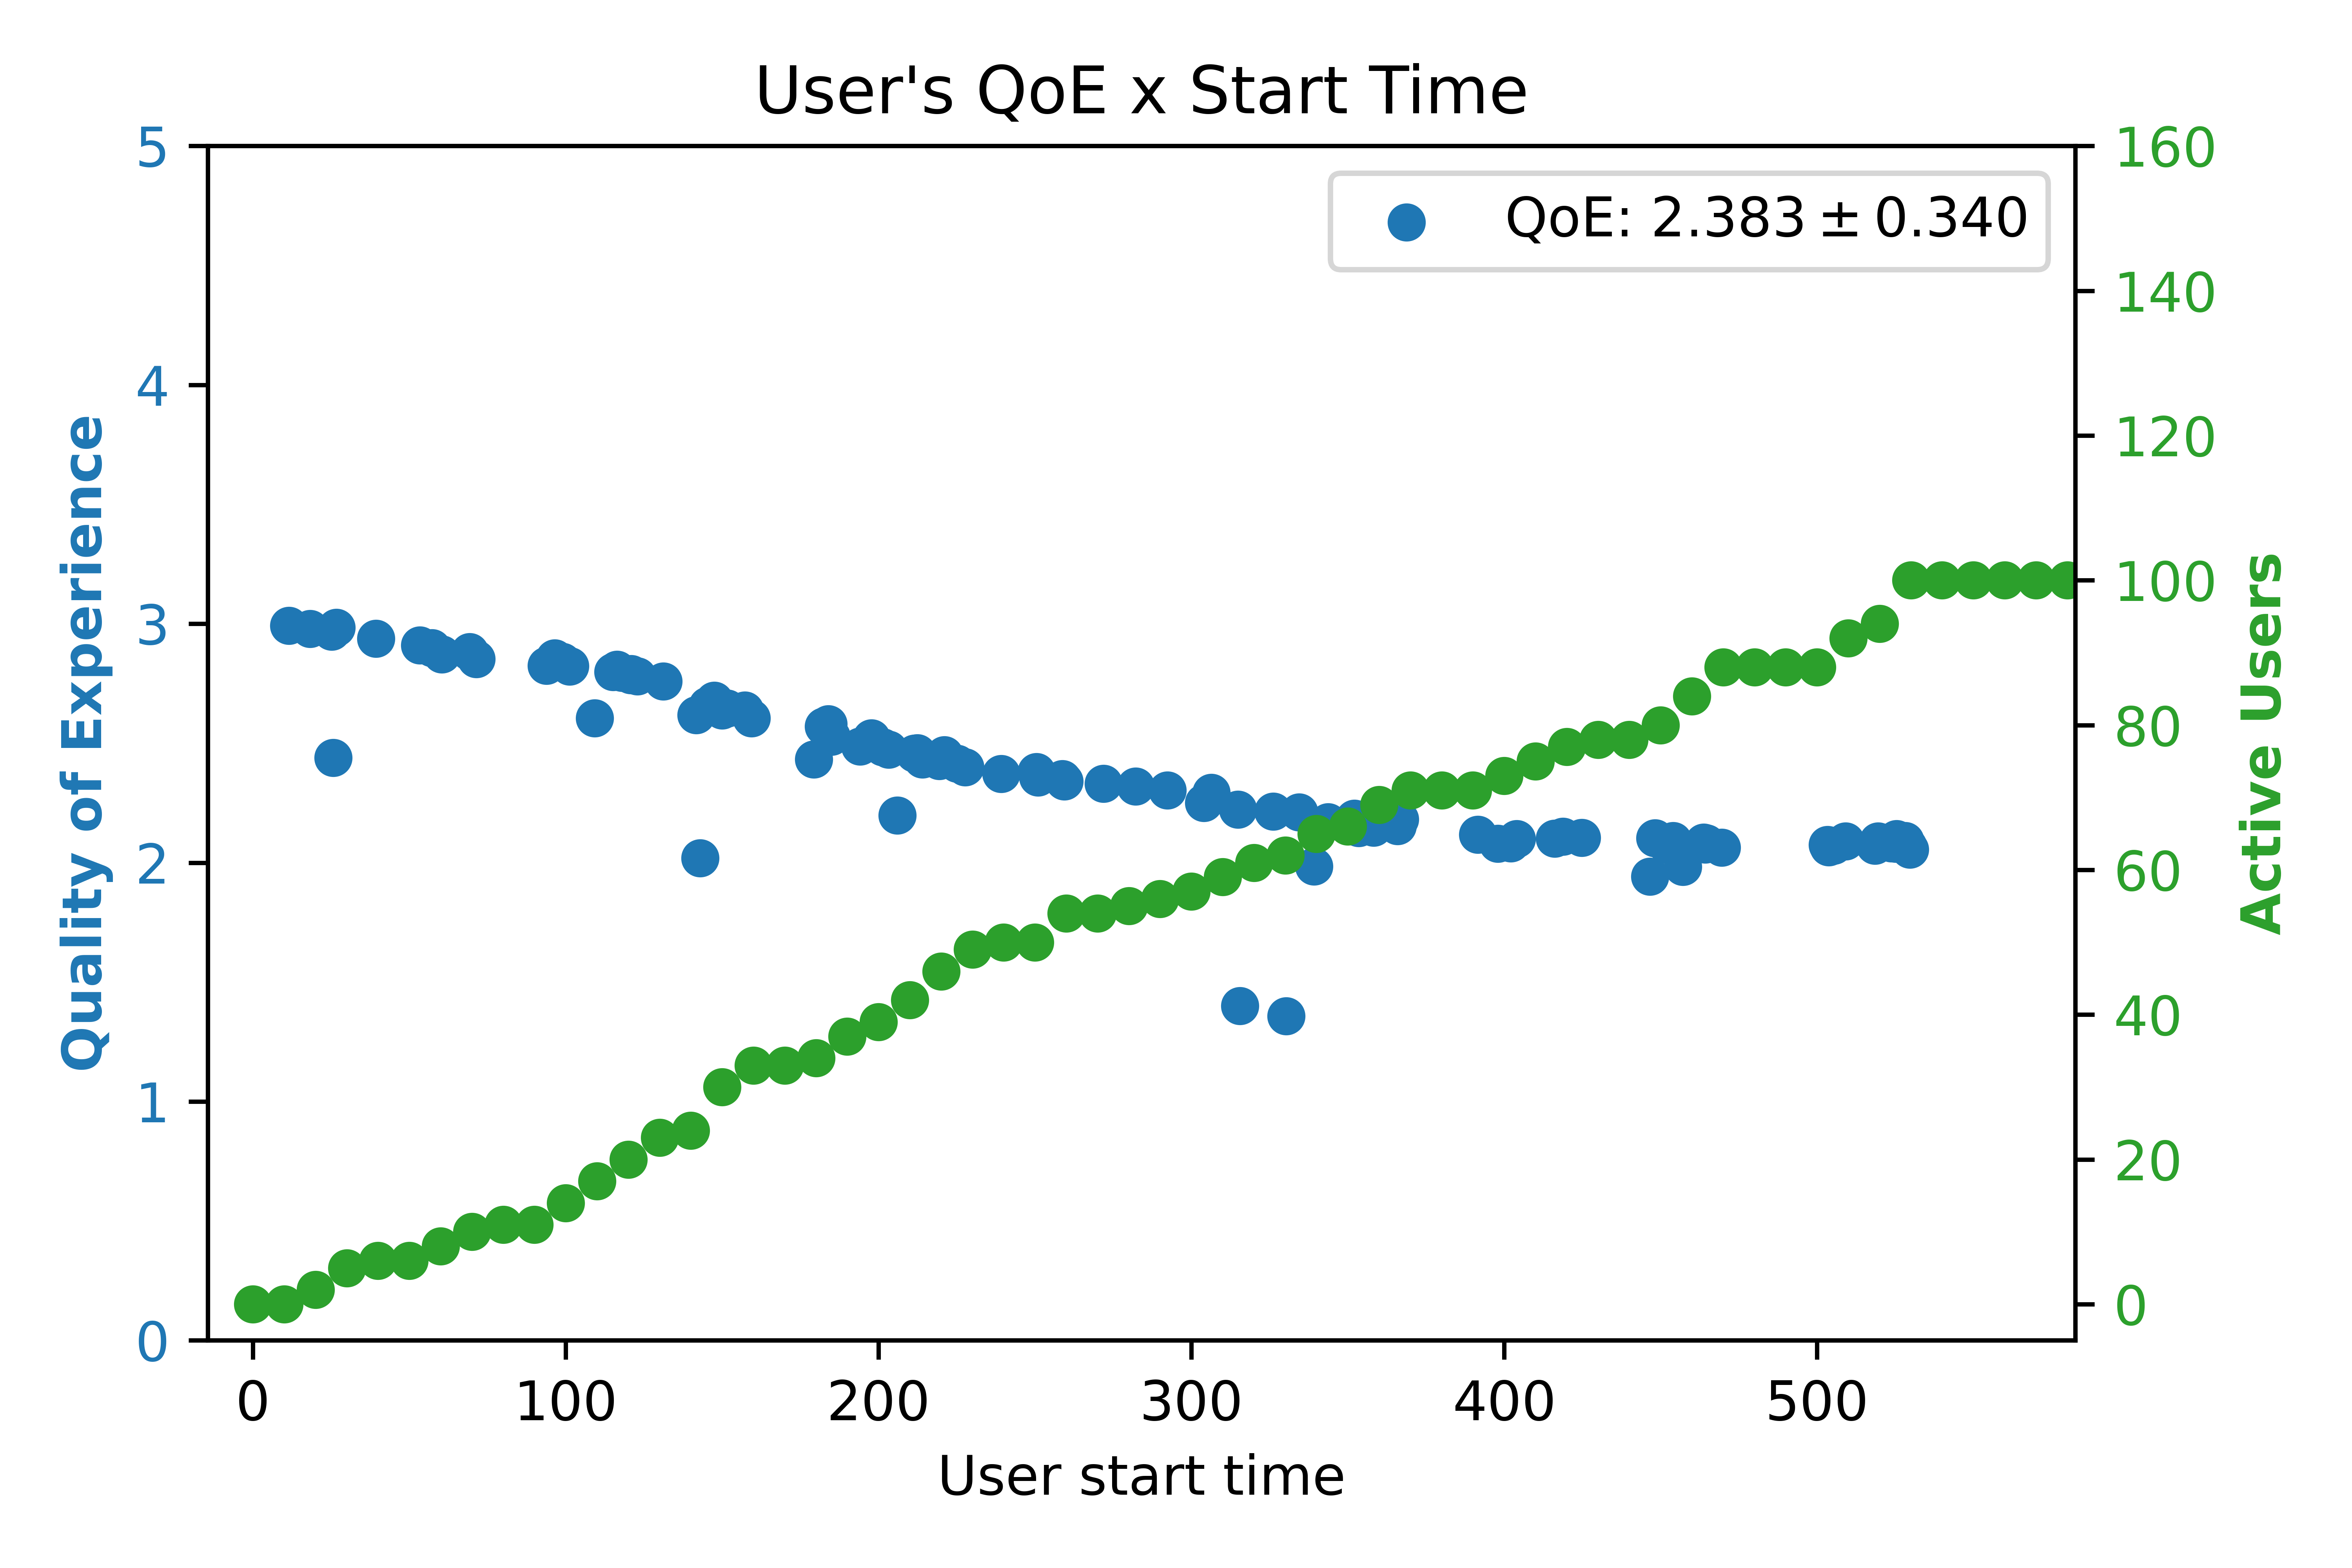
\includegraphics[width=0.31\linewidth]{images/cloud_QoExStartTime25.png}
    \label{fig:plr-comparison-2}
    }
    
    \subfigure[]{
    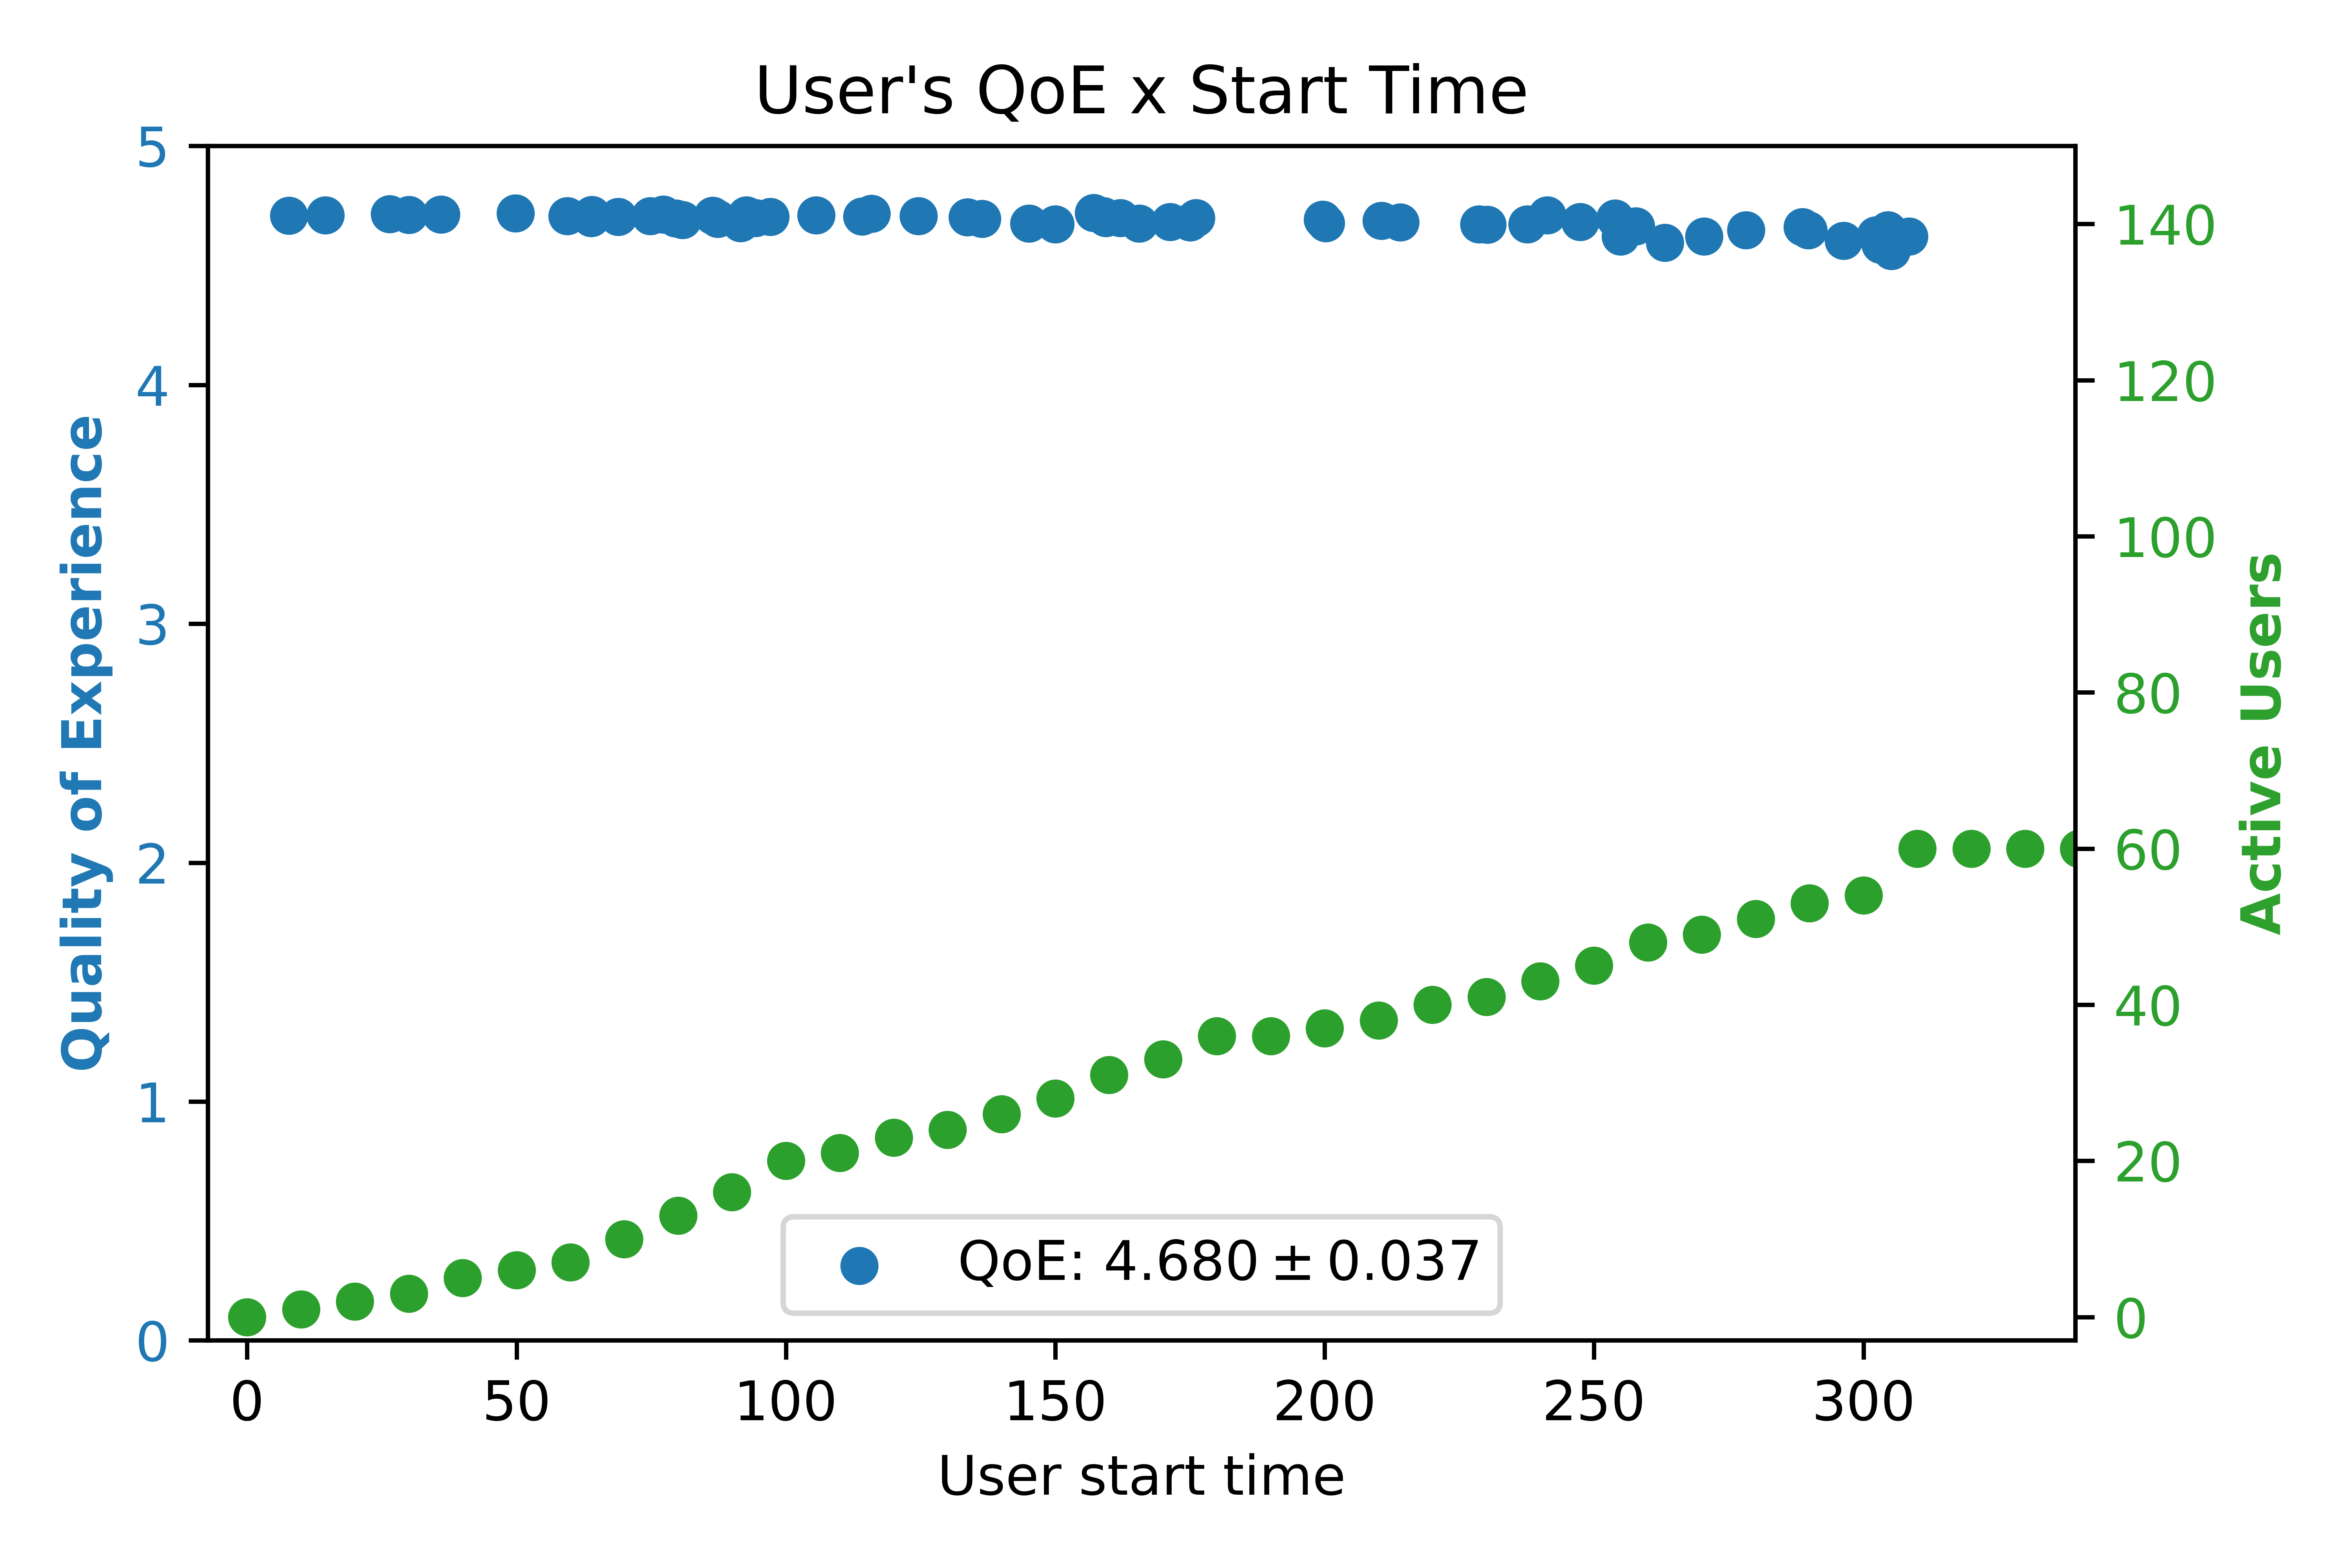
\includegraphics[width=0.31\linewidth]{images/Redicrect_QoExStartTime15.png}
    \label{fig:rssi-comparison-2}
    }
    \subfigure[]{
    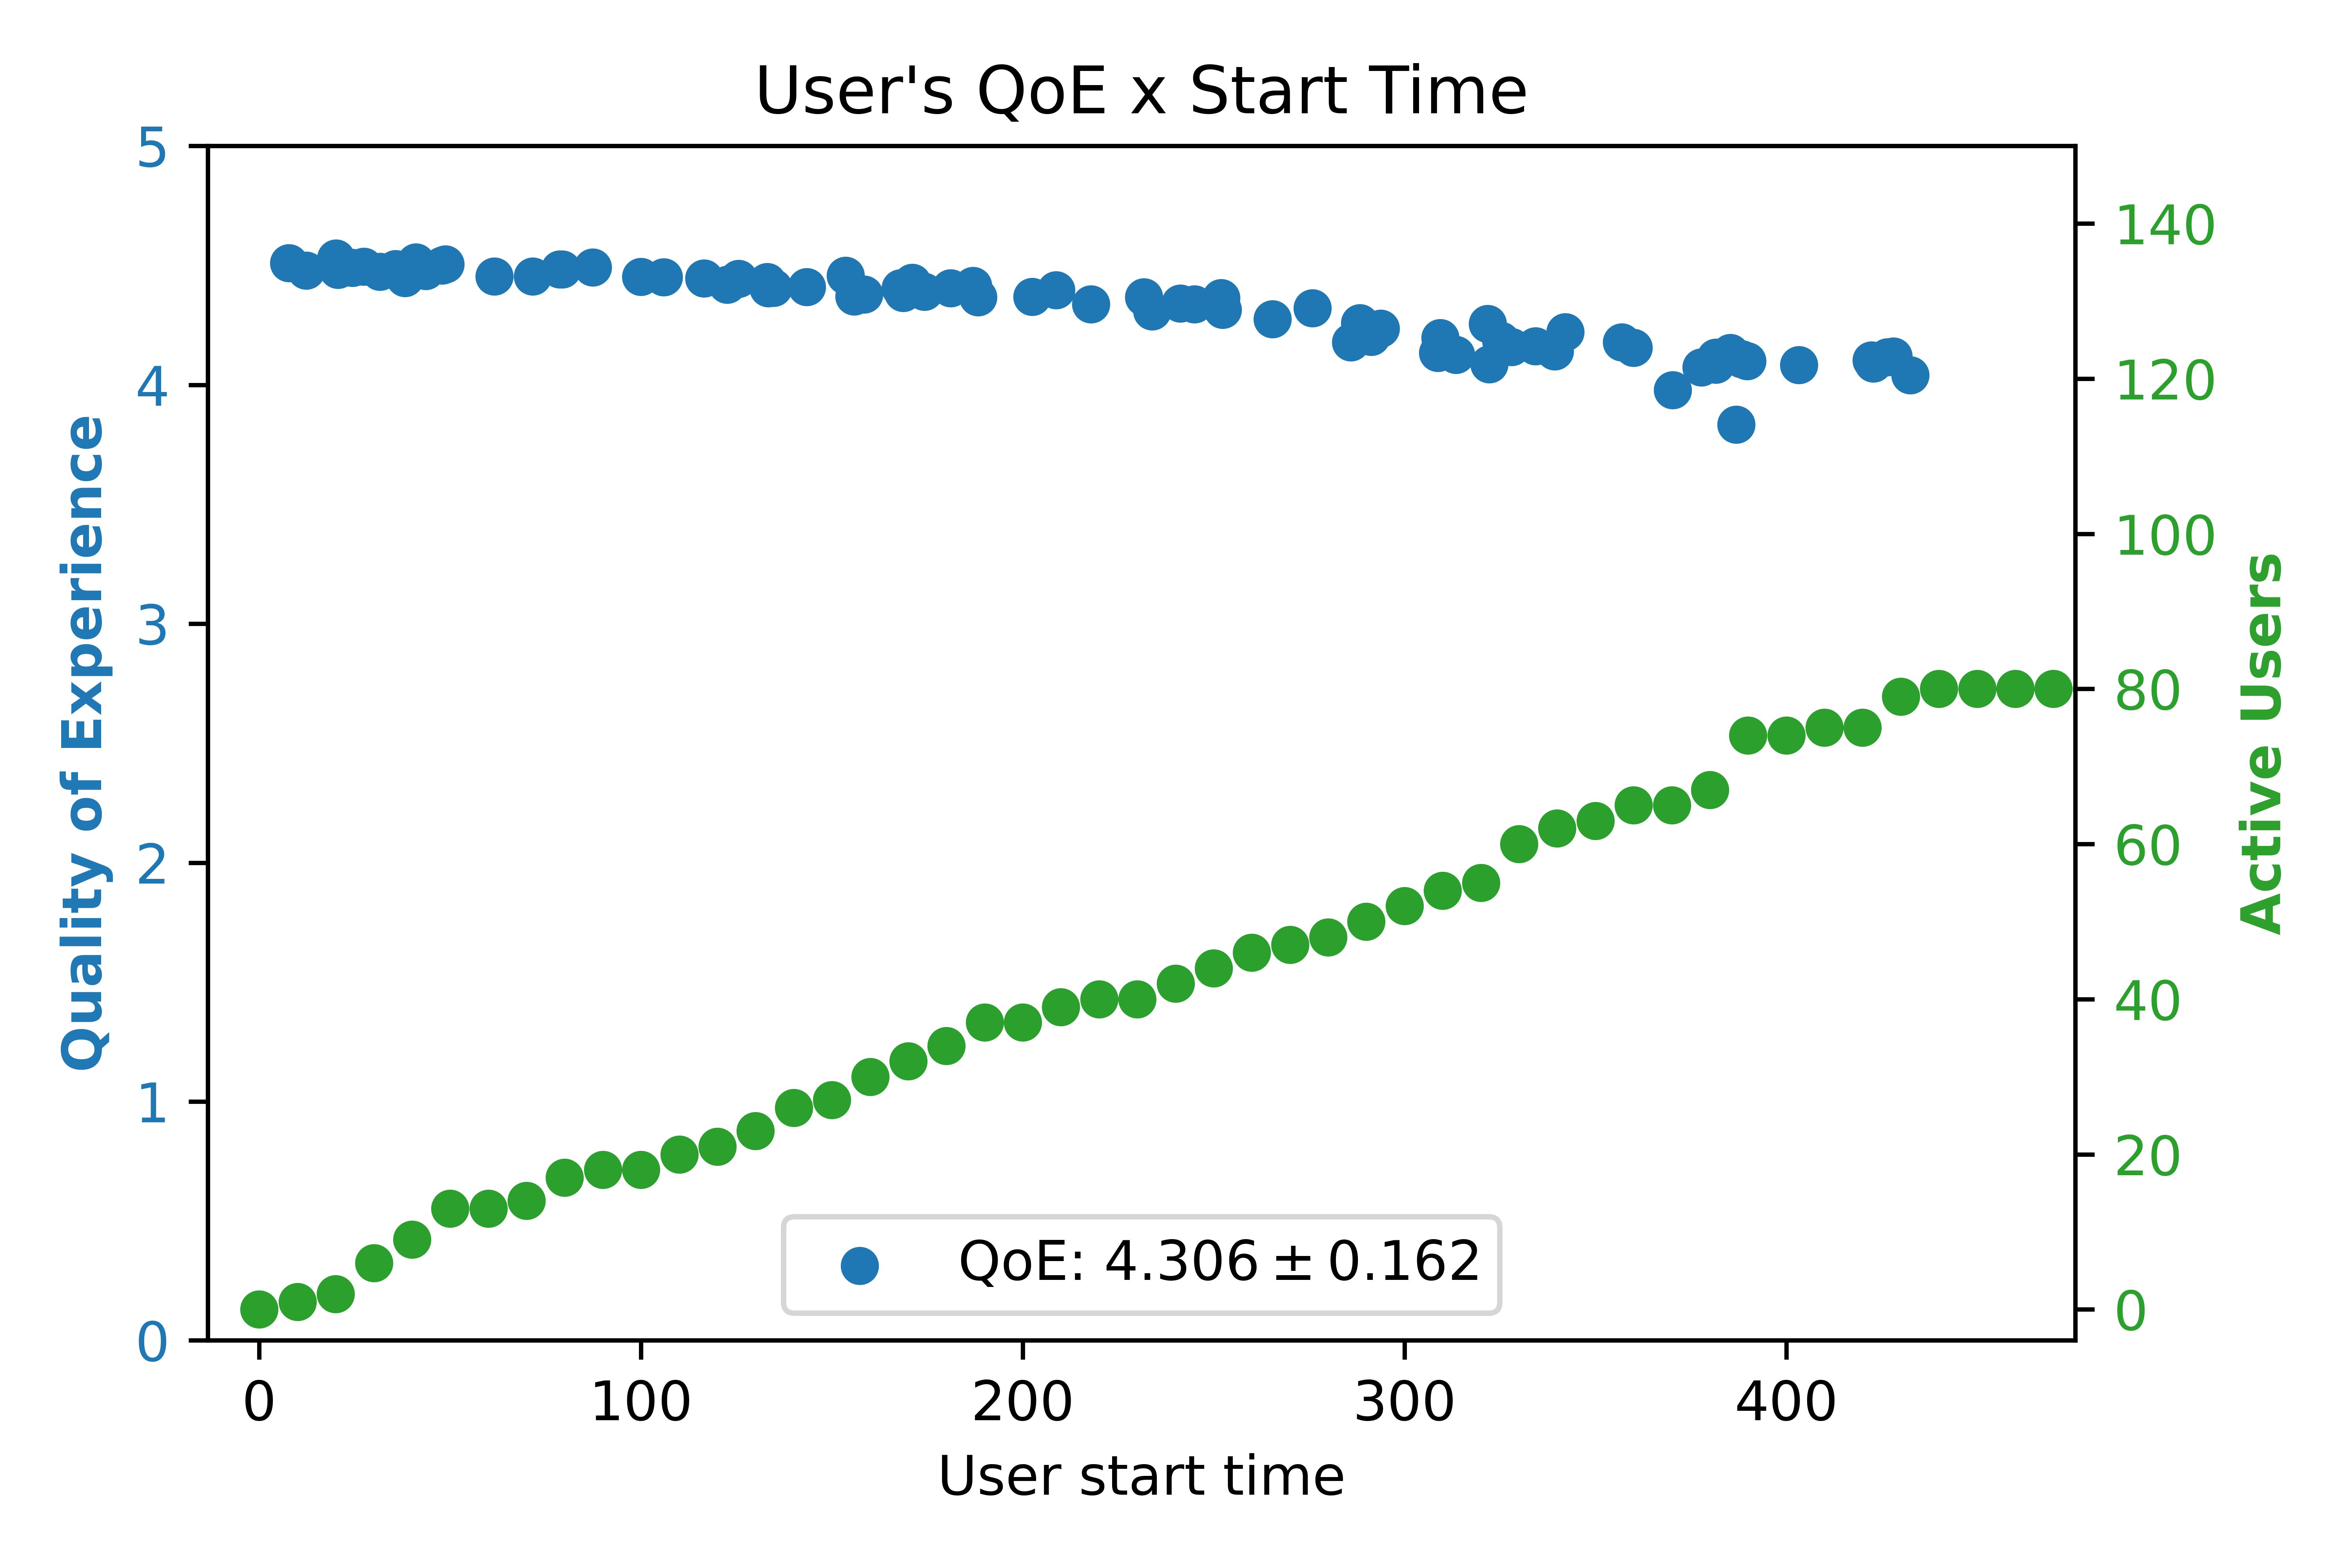
\includegraphics[width=0.31\linewidth]{images/Redicrect_QoExStartTime20.png}
    \label{fig:plr-comparison-2}
    }
    \subfigure[]{
    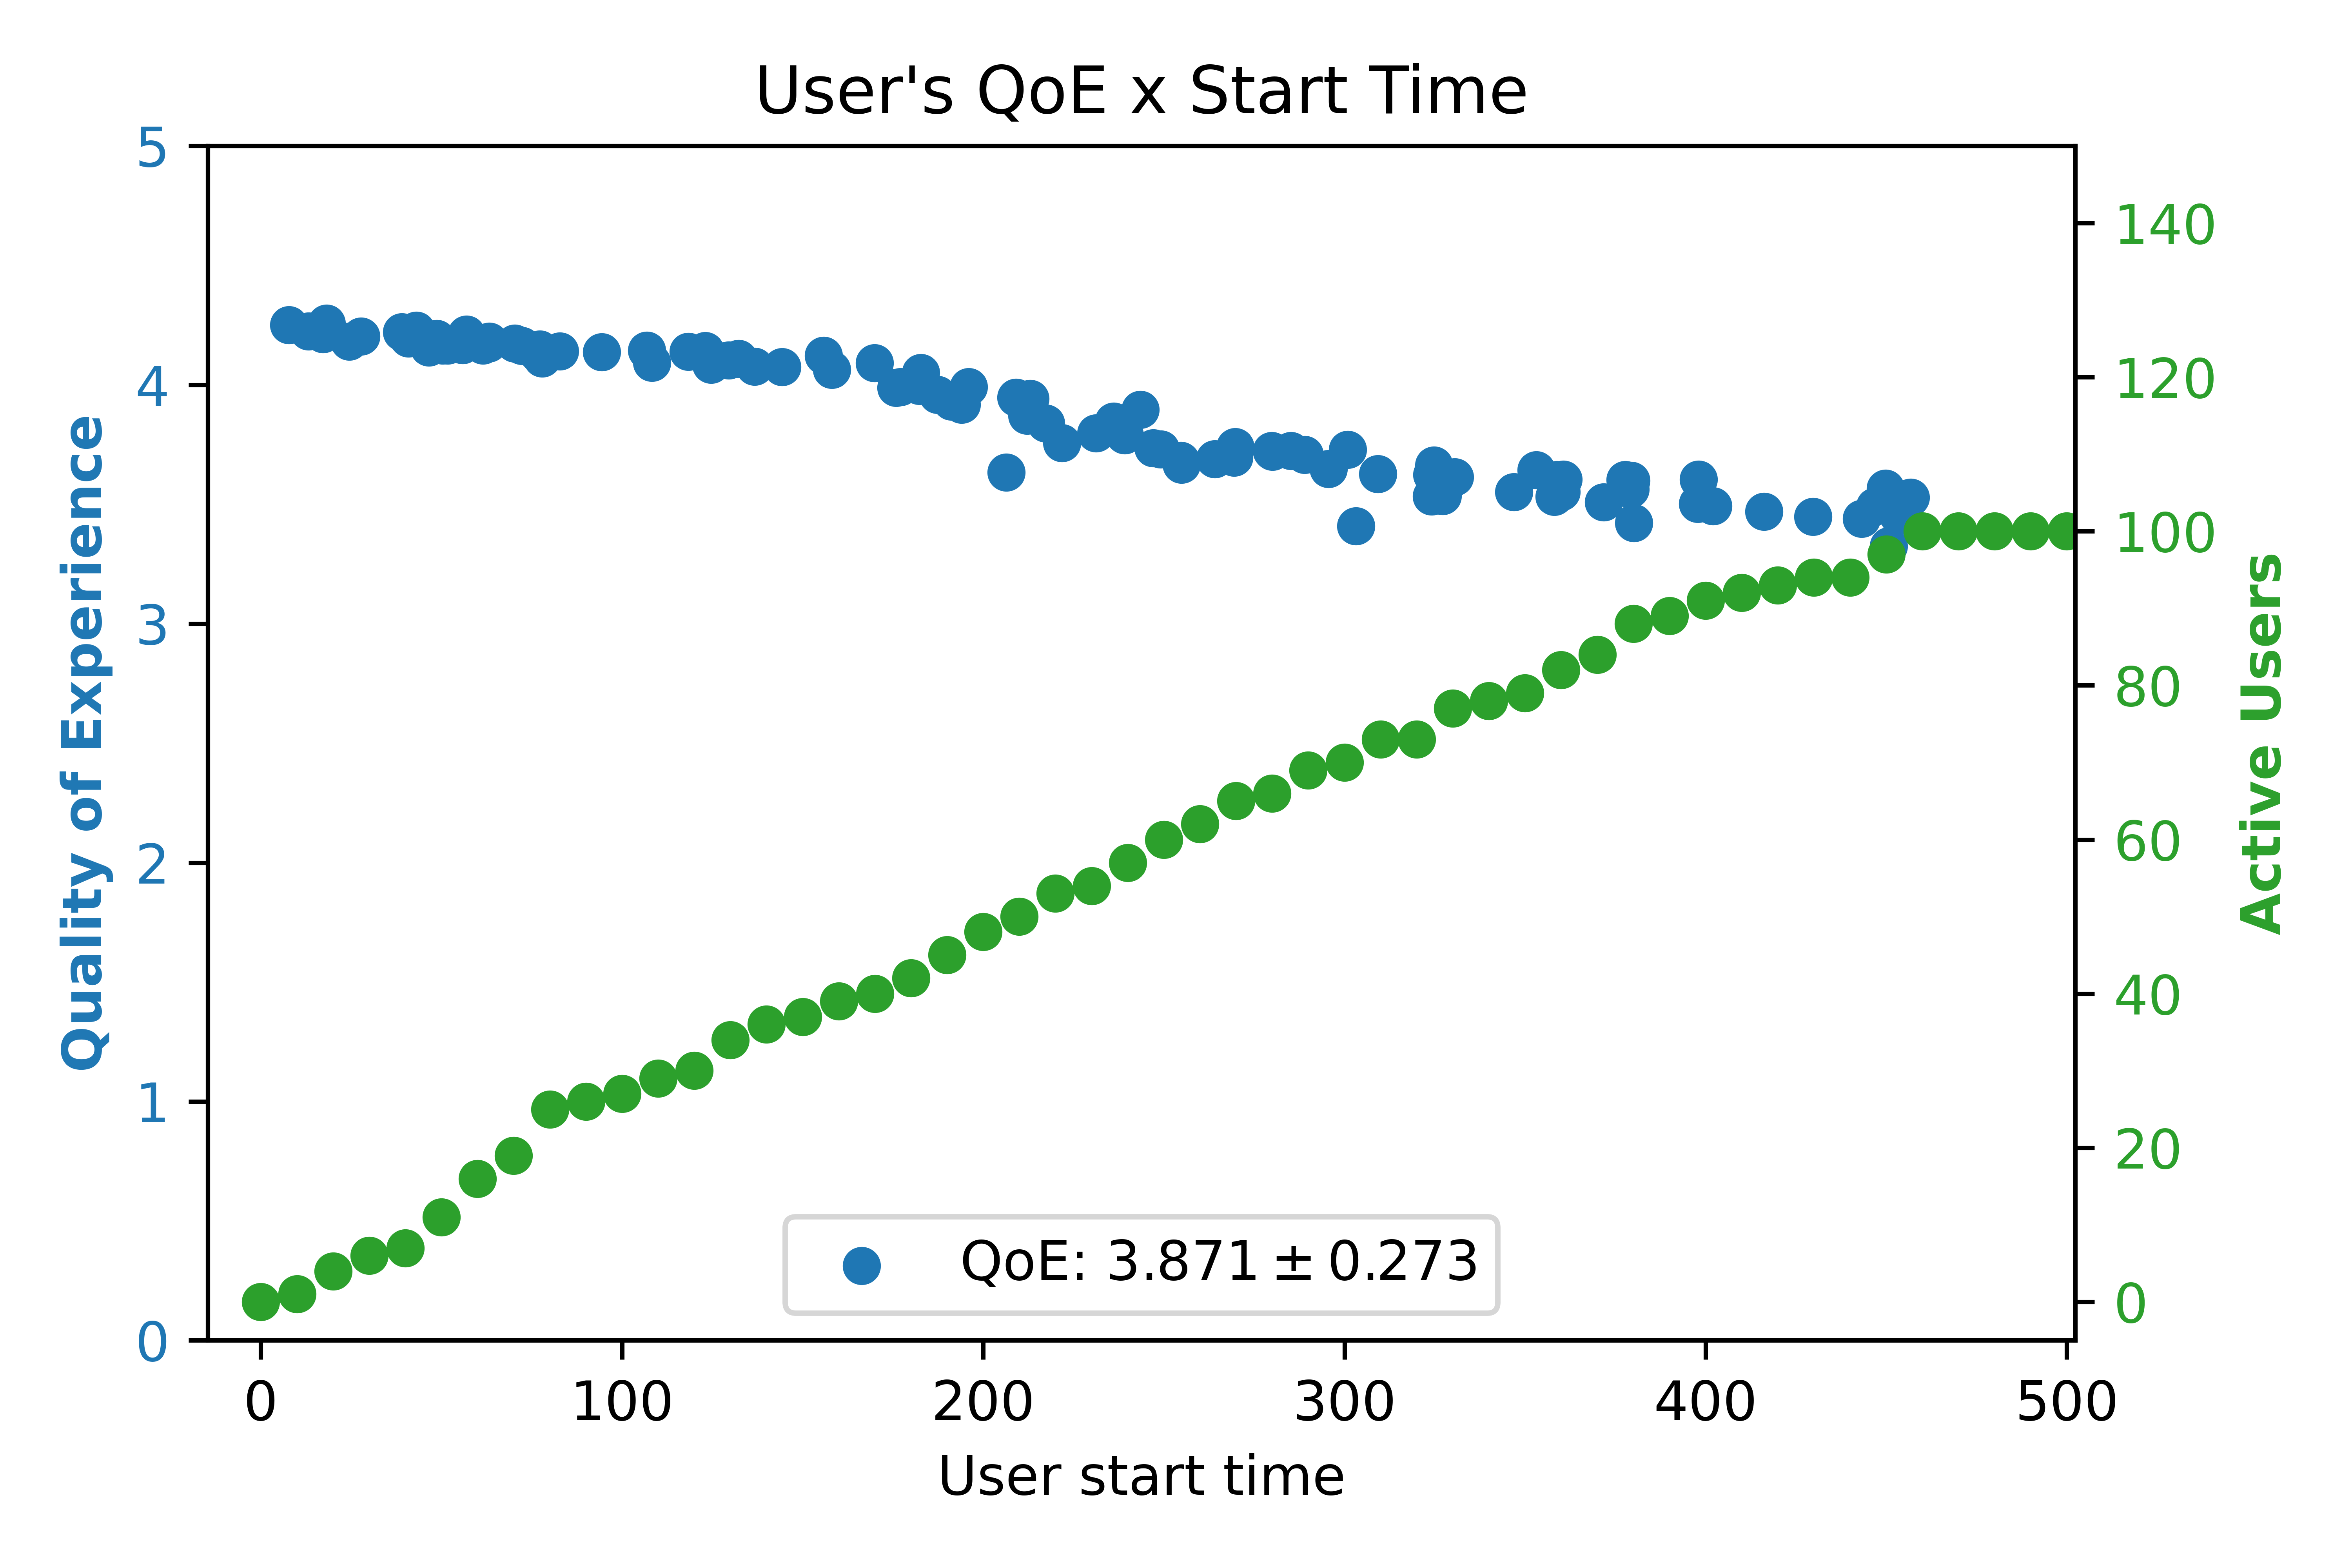
\includegraphics[width=0.31\linewidth]{images/Redicrect_QoExStartTime25.png}
    \label{fig:plr-comparison-2}
    }
    
    \caption{Impact of system on the network performance. Distance \textit{d} between sensor node and antennas of 8m in a semi-NLOS scenario.}
    \label{fig:comparison-qoe-2}
\end{figure*}

\subsection{Discussion and Results Summary}

%As mentioned earlier, the behavior of ABR schemes introduces the problem of selfish decisions when choosing the next segment to be requested. Obviously, different metrics of segment choices lead to different results in the status of buffer occupation and quality of the user's video, which results in a different QoE factor according to the heuristic used.

The experiments illustrated in Figures~\ref{fig:comparison-boxplot} to show the average QoE as shown in~Eq.~\ref{eq:qoe-equation} to 15, 20, and 25 users from left to right, respectively. The boxplot represents the Cloud-only, 1\&2 node and mobility scenarios. As seen, the overall average performance of the 1\&2 is higher than the Cloud-only and mobility. Mainly due to the choices of nodes at the edge peering nodes for serving the requests done by users. 
%
For instance, for a 1\&2 experiment, it occurs congestion in the intermediate links $e_{0,1}$ e $e_{0,2}$, 
the edge peering nodes are activated to serve the end-users below those nodes. In this way, the traffic passing through the link above will now be smoothed out, so the users can improve their resulting QoE to an excellent level.
%edge peering nodes are activates para atender os usuários abaixo desses nós. Desta forma, os trafego que estava passando pelos link acima agora vão ser suavizados, assim os usuários conseguem melhorar seu QoE resultante para um nível excelente.    
%
Since the users request the segments by the closer nodes and with no congestion link in scenarios 1\&2, it is evident that as the QoE increases. %Remember that the scenario 1\&2, there is a link congestion monitoring, so when a congestion link is detected, the cache node above the link is activated, and the users are redirected to request the video from the cache node.
%
The performance difference of the Cloud-only and mobility is near one order of satisfaction for 15 and 20 users and approximately two~three orders of satisfaction with 25 users.


It is important to note that the QoE results of scenarios after mobility are similar to the results of Cloud-only, even that the edge peering nodes using the QoE. This is due to the lack of a rerouting mechanism in real-time when users switch to another AP. The connections between the edge peering nodes and the users remain unchanged, so that the paths through which the packets pass are worse, negatively impacting the performance of the network as a whole.
%Another point to be noted is the average bit rate between different levels. In the scenario with 20 users, level 3 was able to achieve what is necessary to obtain the highest bit rate representation, thus, network operators can seek to deploy caches during peak hours to provide the best user experience.

Figures~\ref{fig:comparison-qoe-2} show the QoE final of each user per the start time~(time to start the segment requests). Here, we can see the final QoE degradation to each user's entrance along the simulation execution. The green plot represents the number of active users simultaneously.  
As users reach the final QoE in this experiment, it tends to be slightly lower than the previous one. When looking at the final QoE delta between users $u_{i}$ and $u_{i + 1}$ seem to be irrelevant, but as we increase the delta, the QoE starts to become considerable different. Through the figure~\ref{fig:co-comparison-boxplot} we can also affirm this behavior, as the number of users increases, the average QoE decreases, and the variation between users increases. Also, note that in the simulation with 25 users per system, the system already shows a degradation in the quality negatively perceived by the end-user.

Based on these observations,
a simple strategy of moving the video to the edge can significantly improve the user's QoE. In this way, the video transmission system can provide user satisfaction qualities and tend to keep them watching the video until the end.
However, if there is no correct management of connections in real-time, we can conclude that the impact introduced by the AP changes can significantly decrease the QoE for mobile users. The user experience can end up getting worse even using the edge of the network. Proper management of multimedia content can be done in which the VoD focus the decision-making in provide a a better QoE for the users changes. A simple content migration within the own edge in a upper tier can solve the problem, as well as realize a rerouting between the active users connections and the server nodes. 

%Based on these observations,
%a simple strategy of moving the video to the edge can significantly improve the user's QoE. In this way, the video transmission system is able to provide user satisfaction qualities as well as they tend to keep them watching the video until the end. 
%Contudo, caso não ocorra um correcto management das conexões em tempo real,  we can conclude that the impact introduced by the AP changes can decrease significantly the QoE for mobile users. A experiencia do usuário pode acabar se tornando pior mesmo usando a borda da rede. Um gerenciamento adequado do conteúdo multimidia pode ser feito de modo que uma simples migração do conteúdo dentro da borda pode solucionar o problema.